\documentclass[11pt,a4paper]{report}

\usepackage{minitoc}
\usepackage{amsthm}
\usepackage{amsmath}
\usepackage{listings}
\usepackage{color}
\usepackage{fancyhdr}
\usepackage{float}
\usepackage{geometry}

\usepackage[utf8]{inputenc}
\usepackage[english]{babel}
\usepackage[style=numeric-comp]{biblatex}
\addbibresource{references.bib}
\usepackage{nomencl}
\usepackage[pdftex,colorlinks=false]{hyperref}
\usepackage[pdftex]{graphicx}
\usepackage{wrapfig}
\usepackage{notes}
\usepackage{watermark}
\usepackage{epstopdf}
\usepackage{sectsty,textcase}
\usepackage{lipsum} 
\usepackage[title]{appendix}
\usepackage{subfig}
\usepackage{siunitx}

\usepackage{color}
 
%New colors defined below
 
%----------------------- FILL IN CORRECTLY  -----------------------
\title{Bachelor Thesis} % choose one of the options
\course{THRESHOLD VOLTAGE \\ REDUCTION OF AN \\ LaAlO\textsubscript{3}-SrTiO\textsubscript{3} FET BY THIN \\DIELECTRICS AND PARTIAL \\COVERAGE}
\university{Twente University.}
\faculty{Faculty of Electrical Engineering, Mathematics and Computer Science (EEMCS)}
\chair{Nano-Electronics}
\author{Bagas Prabowo}
\examcommittee{I.r. A.E.M Smink \\
                Prof.dr.ir. W.G. van der Wiel \\
                Prof.dr. J. Schmitz }

\date{\today} 

\newtheorem{thm}{Theorem}[section]
\newtheorem{cor}[thm]{Corollary}
\newtheorem{lem}[thm]{Lemma}
\theoremstyle{definition}
\newtheorem{defin}[thm]{Definition}

\lstset{ %
basicstyle=\footnotesize,       % the size of the fonts that are used for the code
numbers=left,                   % where to put the line-numbers
numberstyle=\footnotesize,      % the size of the fonts that are used for the line-numbers
stepnumber=2,                   % the step between two line-numbers. If it's 1 each line will be numbered
numbersep=5pt,                  % how far the line-numbers are from the code
backgroundcolor=\color{white},  % choose the background color. You must add \usepackage{color}
showspaces=false,               % show spaces adding particular underscores
showstringspaces=false,         % underline spaces within strings
showtabs=false,                 % show tabs within strings adding particular underscores
frame=single,			% adds a frame around the code
tabsize=2,			% sets default tabsize to 2 spaces
captionpos=b,			% sets the caption-position to bottom
breaklines=true,		% sets automatic line breaking
breakatwhitespace=false,	% sets if automatic breaks should only happen at whitespace
escapeinside={\%*}{*)}          % if you want to add a comment within your code
}
\renewcommand{\bibname}{Recommended Reading}
\DeclareGraphicsExtensions{.pdf,.png}
\dominitoc
 % defined environments for theorem, corollary, lemma and definition

%-------------------------- BEGIN DOCUMENT --------------------------
\begin{document}
\maketitle

\chapter*{Abstract}

This research will present two solutions to reduce the high threshold voltage of such device by making the the LAO layer 4 unit cells thick and by partially covering the STO substrate with LAO effectively making the device percolative. The device will be characterized in both room temperature and at 10K.

Results have shown that the gate voltage does decrease by making the LAO layer thinner. However, gate leakage current becomes too problematic as they exceed 1A. Despite this, transistor operations are still possible with an LAO layer thickness of 4 unit cells. A memristive effect is also observed from the device at room temperature. A shift of gate threshold voltage is seen when the device experience a large negative gate voltage.  At 10K, operation of such device indicates better performance in regard to the on/off  ratio and the subthreshold swing. Gate leakage is observed to be lower at 10K in comparison to room temperature performance. 
A percolative FET has not been fully realized. Simulation study has shown that a metal-insulating transition may be possible by making the LAO layer effectively 3.6 unit cells thick. But investigation towards this device is still worthwhile as such a device may possess a low leakage current.

\newpage
\tableofcontents
\chapter{Introduction}


\section{Motivation}
% Large change in resistance upon small changes in Vgs, 

% It might be possible to create an electrostatically controlled percolation provided that the transistor is at its critical point.

% Critical thicknes of 2DES:3

% Percolation theory exhibits phase transistion. So you can change phase from MIT metal insulating trasistion. 

% Hopefully low current and high on current.

Over the last couple of decades, a large interest has emerged into researching complex oxide materials and their application towards new electronic devices. Research has shown that oxide materials can exhibits unique properties such as high-temperature superconductivity, ferroelectricity, and ferromagnetism that can clearly benefit an electronic device. An excellent example of complex oxide materials that has been researched extensively is the interface between LaAlO\textsubscript{3} (LAO) and SrTiO\textsubscript{3} (STO). In 2004, Ohtomo and Hwang discovered that an epitaxially grown LAO above STO produces a 2D electron gas (2DEG) system \cite{ohtomo_hwang_2004}. A couple of years later, Thiel \textit{et al.} \cite{thiel_2006} discovered that the 2DEG in the LAO/STO interface exist if the LAO layer is at a minimum 4 unit cells (uc) thick and has demonstrate that it is possible to tune the conductivity of the 2DEG by means of an electric field. This has led to further interest into researching the application of the LAO/STO interface so that it can be used as an electronic device such as a field effect transistor (FET). Several reports have shown that this is indeed possible \cite{eerkes_wiel_hilgenkamp_2013,forg_richter_mannhart_2012,hosoda_hikita_hwang_bell_2013} but with an LAO thickness of more than 4 unit cells and a relatively large threshold voltage.

A lower threshold voltage is highly desirable in FET device. To solve this issue, a thin dielectric is often implemented. In this report, we investigate the effect of miniaturizing the LAO/STO based FET. We will examine the consequence of reducing the LAO layer thickness to 4 uc with the goal of reducing the threshold voltage while maintaining acceptable leakage.

From Thiel's \cite{thiel_2006} report, it is concluded that the conductivity at the LAO/STO interface abruptly increases when 4 uc is epitaxially grown onto the STO substrate. This suggests that there a critical thickness exist in which the device is between the insulating and the conducting state. Following this idea, a percolative based field effect transistor is proposed in this report to study the possible metal-insulator-transition behaviour which can be operated at room temperature by field effect. By utilizing this phenomoenon, it is expected that the device will have a low power dissipation due to the low leakage currents from the drain and the gate from altering the state. By making a percolative interface, the effective gate area will also be reduced subsequently reducing the gate threshold voltage.

\newpage

\section{Overview}
The report will be divided into 5 chapters. The content of each chapter is discussed as follow:

Chapter 2 gives an overview over the theory required for this report. The LAO/STO interface and the underlying physics behind it is discussed along with transistor fundamentals. A brief overview of classical percolation theory and random resistor tunneling theory is discussed. The chapter ends with a preliminary discussion on the theory for a top gated 4 uc LAO/STO FET and percolative FET.

Chapter 3 describes the method used to obtain the results presented in this report. The chapter will discuss about the device fabrication, percolation simulation, and the methods used to obtain the I-V characteristic of the oxide transistor under study. 

%Needs to be change since the order will be different.
Chapter 4 reviews the results obtained in this investigation. It is split into mainly 4 parts consisting of room temperature measurement, low temperature measurement, C-V characteristics, mobility and carrier density characteristic, and percolation simulation.

Chapter 5 ends the report with a conclusion and an outlook on what can be researched further.

The appendix will discuss the simulation results in more detail alongside with the framework for simulating random resistor tunneling network. The appendix will also discuss on the results obtained from samples.


\chapter{Theory}

%In the following chapter the LaAlO\textsubscript{3} - SrTiO\textsubscript{3} interface will be discussed. An overview of transistor fundamentals will also be presented in this chapter to give a background for this report alongside percolation theory. This will give a foundation towards the goal of the project being a percolation based field effect transistor.

\section{LaAlO\textsubscript{3} - SrTiO\textsubscript{3} Interface}
LAO and STO are classified as oxide perovskite with a general formula ABO\textsubscript{3}; where A is a type of alkaline earth metal or rare earth metal and B is a type of transition metal or poor metal. In both materials, the perovskite structure has alternating layers of AO and BO\textsubscript{2}. In the case of STO, all layers (TiO\textsubscript{2} and SrO) are electrically neutral whereas in LAO, each layer has a charge of $\pm$e (AlO\textsubscript{2}\textsuperscript{-} and LaO\textsuperscript{+}). The STO and the LAO have a direct band gap of 3.2 eV and 5.6eV respectively \cite{ohtomo_hwang_2004} which classifies them as an insulator. In addition, both materials have a relatively high dielectric constant in comparison to SiO\textsubscript{2}; LAO with a dielectric constant of $\sim$25 and STO with a dielectric constant of $\sim$300 at room temperature \cite{ohtomo_hwang_2004}. Moreover, both materials have similar lattice parameter with STO = \SI{3.905}{\angstrom} \cite{koster_1998} and LAO =  \SI{3.790}{\angstrom} \cite{geller_wood_1956} making it suitable for LAO to be epitaxially grown on top of STO.

The origin of the 2DEG system at the interface of LAO/STO is still widely debated. Initial mechanism proposed by the original publication \cite{ohtomo_hwang_2004} suggest that the conductivity arises from electronic reconstruction. As shown in Figure \ref{fig:Polar Catastrophe} the mechanism is as follows: When LAO is deposited above the TiO\textsubscript{2} terminated STO substrate, polar discontinuity takes place due to the TiO\textsubscript{2} and LaO\textsubscript{2}\textsuperscript{-} interface. As more LAO unit cells are added, an internal potential builds up due to the charged layers (AlO\textsubscript{2}\textsuperscript{-} and LaO\textsuperscript{+}). At 4 unit cells thick, the potential build-up exceeds the band-gap of STO and electronic reconstruction happens where 0.5e\textsuperscript{-} per unit cell from the LAO is transferred to the interface compensating for the diverging potential build-up shown in figure \ref{fig:Polar Catastrophe}b. Another proposed theory is due to oxygen vacancies in the STO \cite{kalabukhov_2007}. A missing oxygen ion will introduce 2 electrons to the system, equivalently doping the STO. However research has claim that this is not necessarily the case due to the contribution of electrons from oxygen vacancies alone would not be enough to achieve the electron density observed from the LAO/STO interface \cite{cantoni_gazquez_2012}. The research concludes that there are several mechanisms involved that describes the physics behind the LAO/STO interface. 

% It is beyond the scope of this report to discuss the different possible mechanisms that may have contribute to this phenomenon, this section is meant as an introductory description that represents the phenomenon.

The 2DEG at the interface possesses very unique properties. Reports have shown that the 2DEG can be electrostatically tuned at both room temperature and low temperature \cite{forg_richter_mannhart_2012} along with signs of ferromagnetism \cite{pavlenko_2012}. Moreover, superconductivity is also achieved at $\sim$310mK and shows that it can be controlled by an electric field \cite{caviglia}. This allows such interface to be tuned to its superconducting state and insulating state. Knowing this, it is clearly appealing to use this materials for new electronic devices by perhaps utilizing its ability to transform between its superconducting state and insulating state.

\begin{figure}
    \centering
    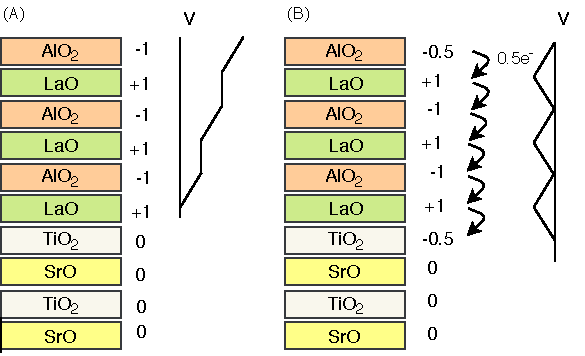
\includegraphics{Figures/Polar_Catastrophe.pdf}
    \caption{Origin of conduction at the LAO/STO interface following the polar catastrophe model.(A) shows the diverging potential due to the alternating charged layers and the polar discontinuity. This is not a physical scenario.(B) shows how this can be possibly resolved. By bringing 0.5e\textsuperscript{-} charge to the interface, potential divergence is averted.}
    \label{fig:Polar Catastrophe}
\end{figure}

%https://codereview.stackexchange.com/questions/178603/compare-neighbors-in-array



% https://www.mrl.ucsb.edu/~vandewalle/complexoxide.php 
%what is the LAO STO interface, What causes it.
% The idea behind the transistor, why would a transistor be interesting.
% Mention why the critical 4uc threshold
% FOund from research paper that the threshold is 4uc Thiel et al.

\section{Field Effect Transistor Fundamentals}
 In principle, the field effect transistor can be thought of as a resistor with a varying resistance that is controlled by a field effect. This section is limited to the description of silicon based metal-oxide-semiconductor field effect transistor (MOSFET) as they are the most common type of FETs whose principle can be applied to similar devices.

% say what an Nmos is, forgot about that.

A typical structure of a MOSFET is shown in figure \ref{fig:MOSFET_Cross-Section}a. The MOSFET is a 3 port device indicated by the drain, source, and gate. There are two common types of MOSFETs namely the nMOS and the pMOS. The operation of the nMOS is practically similar to the pMOS. In figure \ref{fig:MOSFET_Cross-Section}, an n type MOS is illustrated. It is assumed here that the source and the bulk of the MOSFET is connected to ground. 

The operation of an nMOS is as follows: When a positive gate source voltage (i.e V\textsubscript{gs}) is applied, it will repel the holes in the p-type bulk only to leave the acceptor ions. This region of ions under the gate is called the depletion region. Only small amounts of carriers exist in this region. When V\textsubscript{gs} is above a certain threshold voltage, the interface below the gate will start to accumulate electrons. This accumulation of electron will create an inversion layer in which the p-type region under the gate becomes an n-type. The inversion layer is illustrated in figure \ref{fig:MOSFET_Cross-Section}b. Provided that a positive drain-source voltage (i.e V\textsubscript{ds}) is applied, the electrons will flow from the source toward the drain. Naturally, higher voltage at the gate will induce more carriers in the channel increasing the drain current. But this happens only to a certain extent. Saturation will occur when V\textsubscript{ds} reaches V\textsubscript{d,sat} which is defined as V\textsubscript{gs} - V\textsubscript{t}. At saturation voltage the net voltage in the drain side will be smaller than the source side. A further increase of V\textsubscript{ds} will remove the channel at the drain side which only leaves the depletion layer as shown in figure \ref{fig:MOSFET_Cross-Section}c. The channel current will no longer depend on V\textsubscript{ds}. A further increase will only result the pinch off point to move further away from the drain and will not increase I\textsubscript{d}.

\begin{figure}
    \centering
    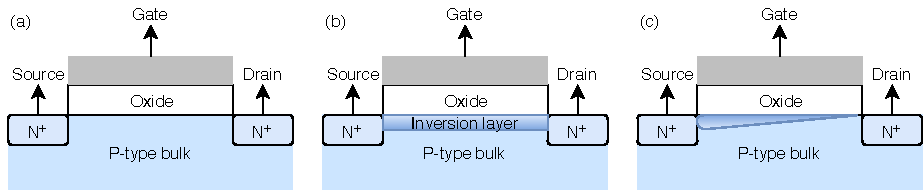
\includegraphics[width = \textwidth]{Figures/MOSFET.pdf}
    \caption{Cross-section diagram of an nMOS. The source and the drain are heavily doped n-type semiconductor. While the substrate is a p-type semiconductor. The oxide maybe SiO\textsubscript{2}. With the gate being a metal or a heavily doped semiconductor.}
    \label{fig:MOSFET_Cross-Section}
\end{figure}

\begin{figure}
\begin{minipage}{.5\linewidth}
\centering
\subfloat[]{\label{fig:MOSFET_Cross-Section_sim_id_vgs}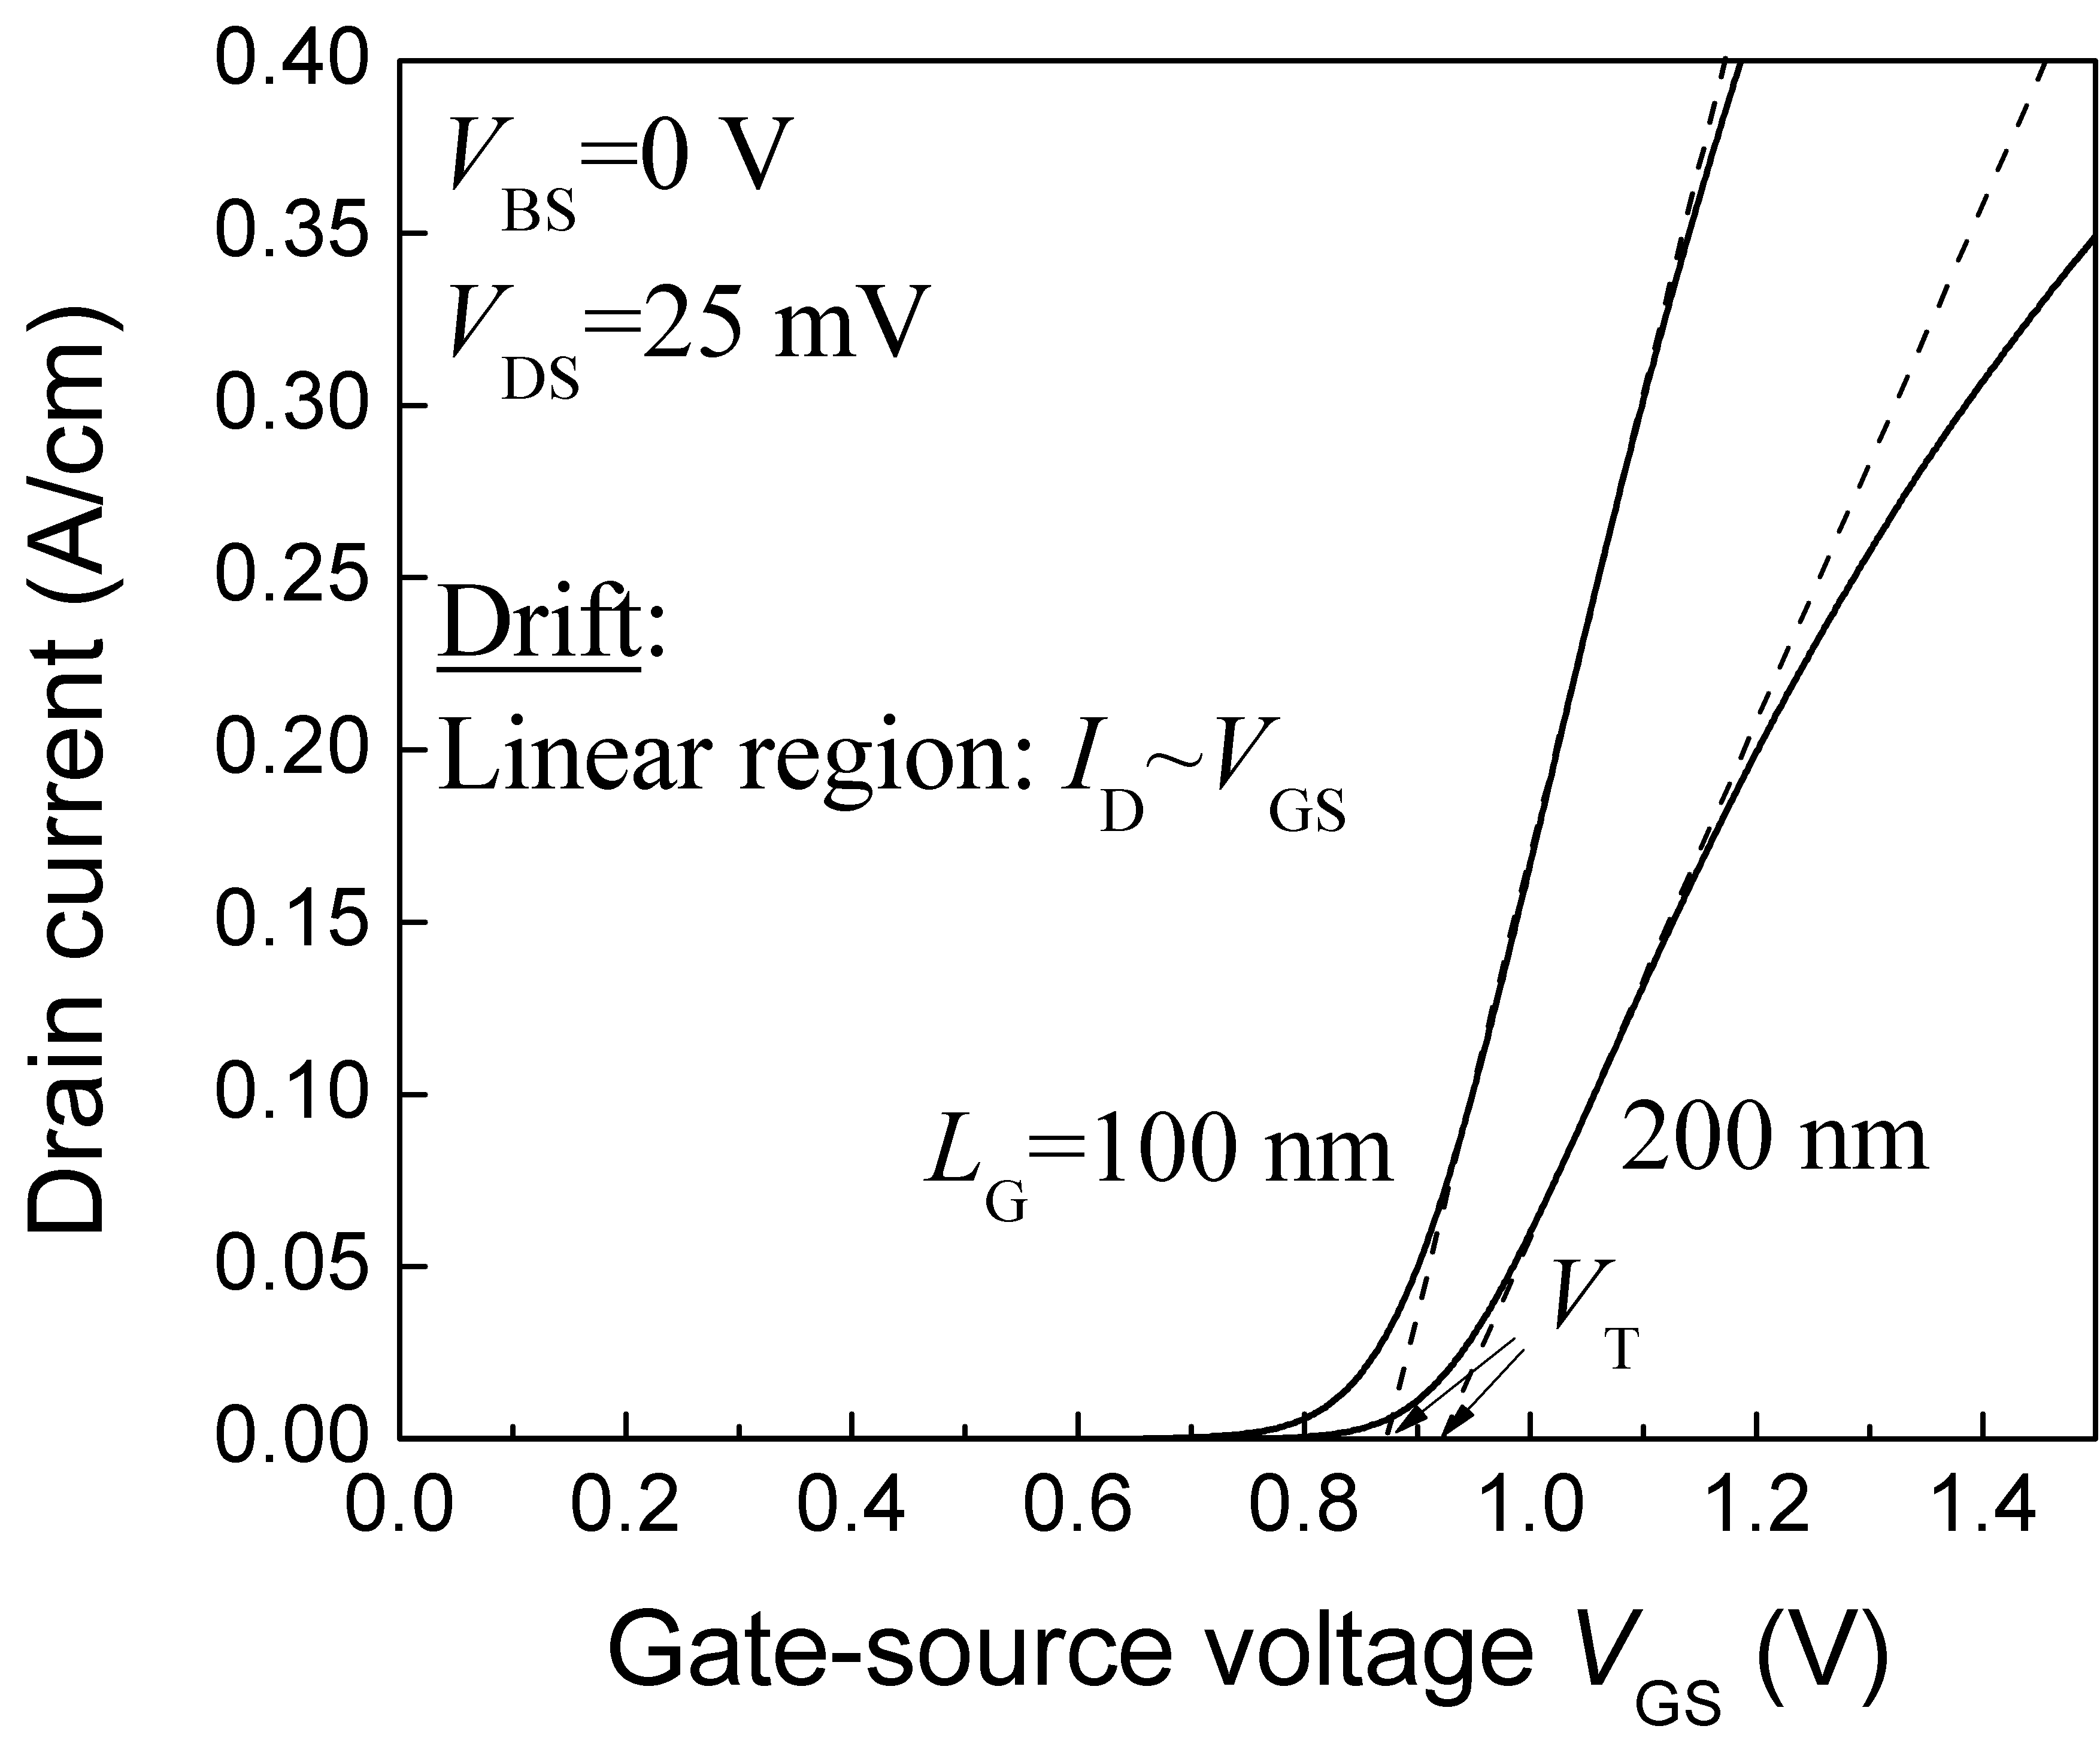
\includegraphics[width = 0.75\textwidth]{Figures/Ids_vs_Vgs_Sim.png}}
\end{minipage}
\begin{minipage}{.5\linewidth}
\centering
\subfloat[]{\label{fig:MOSFET_Cross-Section_sim_id_vds}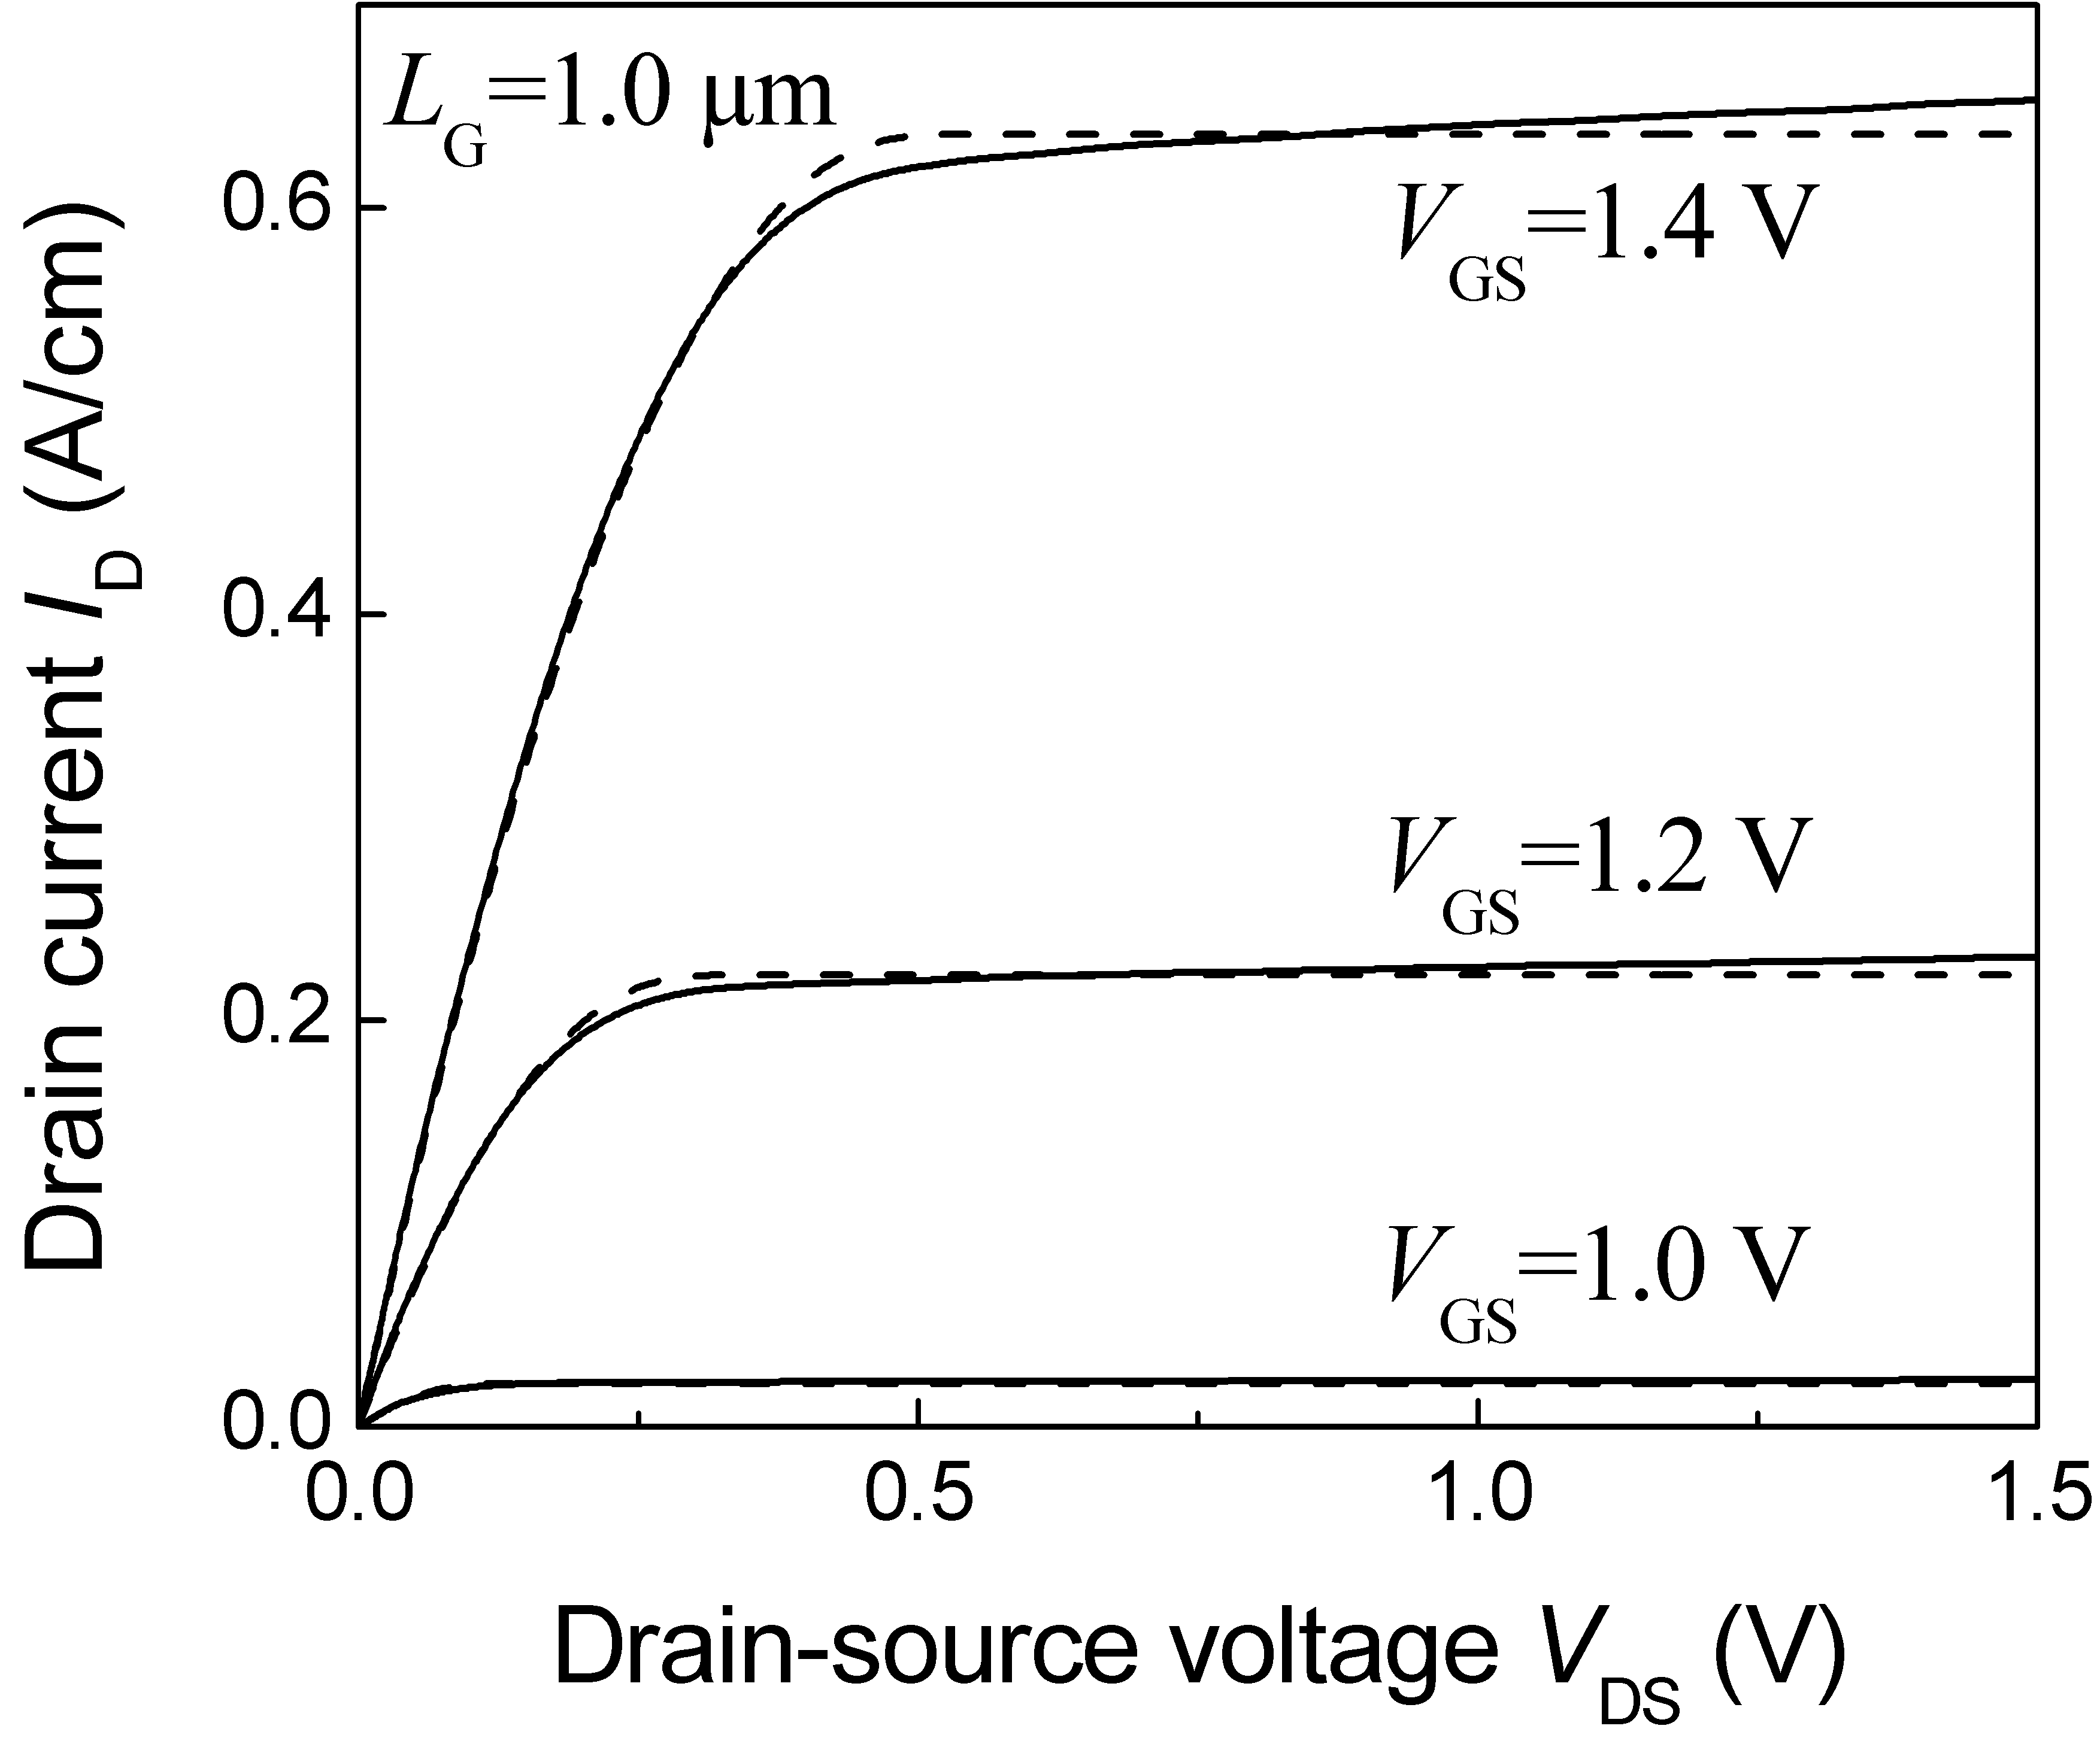
\includegraphics[width = 0.75\textwidth]{Figures/Ids_Vds_Sim.png}}
\end{minipage}\par\medskip
\caption{MOSFET characteristics obtained from simulation.(a) I\textsubscript{d}-V\textsubscript{gs} characteristics for V\textsubscript{ds} = 25mV for gate length of 100nm and 200nm.(b) I\textsubscript{d}-V\textsubscript{ds} characteristics for varying V\textsubscript{gs} for gate length of \SI{1}{\micro\metre}.(Dashed lines indicates simulation data). Reconstructed from Ref \cite{Semiconductor_explained_more}}
\label{fig:MOSFET_Cross-Section_sim}
\end{figure}

Analytically, the behaviour of a MOSFET can be described by equation \ref{eq:MOSFET_quadratic}. Full derivation of this equation is treated in Ref \cite{Semiconductor_explained_more}. The operation of the MOSFET is described in 3 separate parts: the off state, linear/triode region, and saturation region. Following from the equation, figure \ref{fig:MOSFET_Cross-Section_sim} shows the MOSFET characteristics for I\textsubscript{d}-V\textsubscript{gs} and I\textsubscript{d}-V\textsubscript{ds} from simulation and measurement. It should be noted that the dashed lines are results obtained from simulation while the solid lines are measurement data points. For a relatively large MOSFETs, equation \ref{eq:MOSFET_quadratic} and measurement data agrees considerably as shown in figure \ref{fig:MOSFET_Cross-Section_sim_id_vgs} and \ref{fig:MOSFET_Cross-Section_sim_id_vds}. This is not entirely true for MOSFETs channel length under \SI{1}{\micro\metre} as some short channel effects become dominant. One example of this effects is the channel length modulation. The saturation region shown in figure \ref{fig:MOSFET_Cross-Section_sim_id_vds} will no longer be flat. Instead, it will monotonically increase due to the decreasing channel length with higher V\textsubscript{ds}. This effectively lowers the channel resistance which will increase I\textsubscript{d} even in saturation.

\begin{align}
     I_{d} &=
  \begin{cases}
   0        & \text{; if V\textsubscript{gs}} < \text{V\textsubscript{t}} \\
   \mu_n C_{ox}\frac{W}{L_{ch}}\left(V_{gs} - V_t - \frac{V_{ds}}{2}\right)V_{ds} & \text{; if V\textsubscript{gs}} \geq  \text{V\textsubscript{t}, V\textsubscript{ds}} <  \text{V\textsubscript{g}-V\textsubscript{t}} \\ 
   \mu_n C_{ox}\frac{W}{L_{ch}}\left(V_{gs} - V_t\right)^2 & \text{; if V\textsubscript{gs}} \geq  \text{V\textsubscript{t}, V\textsubscript{ds}} \geq \text{V\textsubscript{g}-V\textsubscript{t}}
  \end{cases}
  \label{eq:MOSFET_quadratic}
\end{align}

In addition to the I-V characterization of the FET, it is also important to characterize other properties of the device such as the sub-threshold swing and the on-off ratio. These parameters would measure how well the MOSFET performs regarding how quick it can generate a channel and how well it can suppress leakage current. Gate capacitance can also determined which gives values for depletion region thickness, mobility, and carrier density.

The sub-threshold swing is defined in equation \ref{eq:subthreshold-swing} \cite{hu_2010}. This value quantifies how large of a V\textsubscript{gs} is needed to change I\textsubscript{d} by one order of magnitude. Theoretically, for a regular semiconductor MOSFET, this is limited to \SI{60}{\milli\volt}/dec at room temperature. This strictly limited by the C\textsubscript{ox} term when it is very large. It is desirable to have a low sub-threshold swing as it means that with a small voltage change, it will change the current by one order of magnitude.

\begin{align}
    S_{s-th} = \ln{(10)}\frac{kT}{q}\left(1+ \frac{C_0}{C_{ox}}\right)
    \label{eq:subthreshold-swing}
\end{align}

The on-off ratio is also an important parameter to look at. This can be readily obtained from I\textsubscript{d}-V\textsubscript{gs} characteristics.  This figure of merit defines the ratio of drain current when the device is at off state and at the on state. Naturally, a low leakage current is desired. In effect, a high on/off ratio is achieved.

\newpage

\section{Percolation Theory}
In this section, percolation theory is introduced and will serve as a foundation to understand the effect of partially covering STO substrate with LAO. The random resistor tunneling network theory is also introduced to explain the possibility of the device being able to change from a metallic state to an insulating state.
\subsection{Classical Percolation Theory}\label{section:Classical Percolation Theory}
\begin{figure}[!b]
\begin{minipage}{.5\linewidth}
\centering
\subfloat[]{\label{fig:non-RRTN_sample}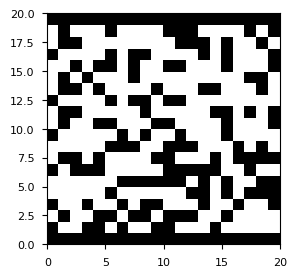
\includegraphics[width = 0.75\textwidth]{Figures/non_RRTN_sample.png}}
\end{minipage}
\begin{minipage}{.5\linewidth}
\centering
\subfloat[]{\label{fig:RRTN_Sample_Section2}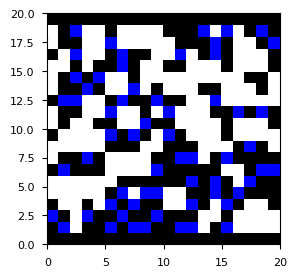
\includegraphics[width = 0.75\textwidth]{Figures/RRTN_Sample.png}}

\end{minipage}\par\medskip
\caption{20x20 Sample with $p$ = 0.4. (a) Non-RRTN sample. (b) RRTN sample.}\label{fig:Simulation Sample figure}
\end{figure}

\begin{table}[!b]
\centering
\begin{tabular}{|c|c|c|}
\hline
Lattice       & Site Percolation & Bond Percolation \\ \hline
1D            & 1                & 1                \\ \hline
2D Honeycomb  & 0.6962           & 0.65271          \\ \hline
2D Square     & 0.592756         & 1/2              \\ \hline
2D Triangular & 1/2              & 0.34729          \\ \hline
\end{tabular}%
\caption{Table of $p_c$ for 1D and 2D lattice. Each configuration gives different $p_c$, most of which are obtained numerically.\cite{christensen_2002}}
\label{tab:Percolation_dimension}
\end{table}

Percolation theory in statistical physics is a theory that describes the characteristics of large lattices with probabilistic occupied sites. Percolative system will have a tendency to display a phase transition, meaning that their macroscopic behaviour changes without any change to their microscopic behaviour. Characteristics of the sample such as mean cluster size, number of clusters, and phase transition threshold can be obtained from the theory and can be used alongside other physical phenomena to explain the critical behaviour of the sample. This phase transition can be influenced by parameters such as temperature, external magnetic field, or occupation probability\cite{Stauffer_classical_percolation_2009}. 

%Explain site percolation
%This is a typical phenomenon in nature for a system with infinite number of degrees of freedom.


An example of a site occupied percolative system is shown in figure \ref{fig:non-RRTN_sample}. In the figure, black pixels indicates occupied sites whereas white ones are not. In the context of this report, each black site can be regarded as a metallic island. Based on figure \ref{fig:non-RRTN_sample}, each site has a certain occupation probability $p$. This is equivalently the concentration of sites in a given sample. The probability of a spanning cluster $P_s$ can also be defined. This value quantifies the probability of whether there exist a cluster which spans from one side of the sample to the other. In the case of an infinite lattice, there exists a well defined percolation threshold probability $p_c$ in which for $p>p_c$ there exist an infinite spanning cluster ($P_s$ = 1). This indicates a phase transition where the sample would suddenly be conducting from one end to another given that the concentration of the site of the sample is above $p_c$. It should be noted that there  are currently no analytical solution for $p_c$ of a 2D square site percolation. The table \ref{tab:Percolation_dimension} summarizes known solutions for the threshold probability for 1 and 2 dimensions. 


\subsection{Random Resistor Tunneling Network} \label{section:RRTN}


Coupled with percolation theory, the random resistor tunneling network (RRTN) theory provides a way to describe the the electrical conductivity behaviour of the sample in a semi-classical way. In RRTN, it assumes that quantum tunneling may occur between two islands. Additional assumptions are added to the percolation theory in such that (i) tunneling can take place between two metallic islands separated by an insulator gap and (ii) the potential barrier in the nearest insulating gap between two metallic islands is constant \cite{Stauffer_RRTN_2009}. As tunneling current falls off exponentially, the tunneling will have a certain upper cut-off distance in which tunneling current becomes negligible. Hence the dimensions of the grid would need to be taken into account whether the RRTN mechanism exist or not.

Figure \ref{fig:RRTN_Sample_Section2} shows the same sample when RRTN is considered. It is clearly observed that there exist a percolative path in the y direction that does not exist in the non-RRTN sample. By considering RRTN, the system effectively has a lower $p_c$. Additionally, the theory can consider the non-linear tunneling behaviour by considering a non-linear piece-wise function to describe the current flowing through neighbouring sites gapped by an insulating sites. For simplicity the function can be thought of as a diode-like function described by equation \ref{eq:linear piece} and shown in figure \ref{fig:piecewise-function}.

\begin{align}
     I_{t} &=
  \begin{cases}
        -\alpha V + \beta & ; V \leq -V_{t,RRTN}\\
        0 & ; -V_{t,RRTN} < V \leq V_{t,RRTN} \\
        \alpha V + \gamma & ; V > V_{t,RRTN}
  \end{cases}
  \label{eq:linear piece}
\end{align}

\begin{figure}
    \centering
    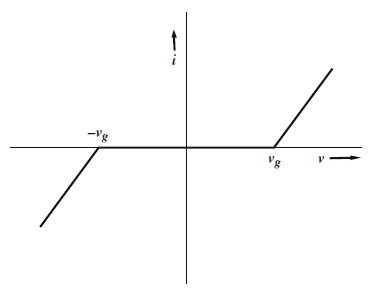
\includegraphics[scale = 0.9]{Figures/Piecewise-function.png}
    \caption{I-V characteristics of the tunneling bond. Reproduced from Ref \cite{Stauffer_RRTN_2009}.}
    \label{fig:piecewise-function}
\end{figure}

Physically, the non-linearity arises from the lowering of potential barrier between each island which leads to a higher current. The constant $\alpha$ is expected to be temperature and barrier energy dependent. The voltage in equation \ref{eq:linear piece} is defined as the potential difference between the top and bottom of the sample. Hence, with this theory, metal-insulator-transition can be explained by modulating the voltage across the sample.


\section{Top Gated LAO/STO FET}
In combination with the knowledge from percolation theory and LAO/STO interface, the 4 uc LAO/STO FET and the percolation FET (perFET) will now be discussed. The oxide based FET is shown in figure \ref{fig:perFET crosscut}. At V\textsubscript{gs} = 0, there exist a conducting channel (shown by the blue layer) under the gate. The FET itself is classified as an n-type depletion mode FET since a negative V\textsubscript{gs} is needed to deplete the electron channel at the interface.

One of the problem with the LAO/STO interface is that it has a high carrier density. On a typical LAO/STO interface, it was found that the carrier density of the interface is approximately in the order of $10^{13}$ \si{cm^{-2}} \cite{thiel_2006}. This would require high electric field to completely deplete it. Hence a low carrier density is clearly desired. One way deplete such a device is to locally tune the 2DEG by top gating. Several studies have shown that this is possible and more favorable in comparison to back gating \cite{forg_richter_mannhart_2012,caviglia}. This is due to the fact that it results a lower gate voltage requirement to deplete it as the 2DEG is closer to the gate and it does not require the gate to fully deplete the 2DEG globally. The threshold voltage can be reduced further by utilizing a thin dielectric. LAO layer of 4 uc thick can be used in this device which will hopefully reduce the threshold gate voltage. Besides optimizing the structure, minimizing the oxygen defects during the fabrication process can also be done. Doing so would reduce the amount of electrons due to oxygen vacancies. This can be done by annealing the sample under an appropriate oxygen pressure after deposition. Another theoretical way to do this is by making the LAO/STO interface percolative. 

In the case of a 4 uc FET, the thickness of the LAO layer is comparable to the state of the art MOSFET dielectric thickness at around $\sim$1.5\si{nm}. Hence a comparative study can be done to quantify the performance difference between the two. The I-V characteristics of the proposed oxide FET here can also be compared to other studies with thicker LAO layer \cite{eerkes_wiel_hilgenkamp_2013, hosoda_hikita_hwang_bell_2013, forg_richter_mannhart_2012}. 

From figure \ref{fig:perFET crosscut} the gate does not extend to both the drain and the source electrode unlike the MOSFET. This is because unlike the MOSFET, the 4 uc LAO/STO FET has a 2DEG channel intrinsically. To turn it on or off, it simply needs deplete the 2DEG under the gate to effectively disconnect the channel between the two electrodes. A change of behaviour in the saturation region might also happen since the gate does not cover the whole 2DEG. This means that the pinch-off point would behave differently than those of a MOSFET.

The realization of a perFET is motivated by the possibility of triggering a metal-insulator-transition of the device in room temperature by field effect. In theory, this could enhance the on/off performance of such FET but perhaps in expense of a lower I\textsubscript{d}. This is because as the mobility of the electrons would considerably be lower in the perFET due to the scattering of the electrons by the non-homogeneous interface. An effectively smaller gate area would also mean that a lower threshold voltage can be achieved. Moreover, the performance of the sub-threshold swing is expected to be lower than 60mV/dec at lower temperature due to the reduction of the temperature and possibility of a negative quantum capacitance \cite{li_Large_capacitance_enhancement_2011}.



%https://phys.org/news/2015-04-negative-electronic-compressibility-material.html negative compressibility

\begin{figure}
    \centering
    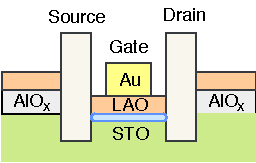
\includegraphics[scale=1.25]{Figures/CrosscutPerfet.pdf}
    \caption{Cross-cut of an LAO/STO based transistor. Blue layer shows the 2DEG layer generated by the LAO/STO interface.}
    \label{fig:perFET crosscut}
\end{figure}


\chapter{Method}

\section{Device Fabrication}
In the following section, the fabrication process is discussed along with the parameters used during the fabrication. Several critical steps are described in details in the following sections.

Device fabrication of the LAO/STO transistor is explained as follows: The STO will be the substrate of the device. The STO is terminated at the TiO\textsubscript{2} layer as shown in figure \ref{fig:fabrication_perfet}A because only then it gives a conducting channel when an LAO is grown on top of it \cite{ohtomo_hwang_2004}.  An amorphous AlO\textsubscript{x} is then deposited using pulsed laser deposition (PLD) at room temperature and oxygen pressure of $2\times10^{-1}$ mbar. This will act as an insulator to separate the deposited layer of LAO later on. Photoresist is added next for patterning. By using UV lithography, a pattern is formed on the sample. Acetone is then used to remove the photoresist leaving behind the patterned amorphous AlO layer. The result of the patterning is shown in figure \ref{fig:fabrication_perfet}E. 

The LAO layer will then be deposited by PLD. The STO substrate will be heated to 850 degrees to ensure sufficient surface diffusion of the arriving LAO particles. The deposition is done under $1\times10^{-4}$ mbar of oxygen pressure. The laser fluence was \SI{1.3}{\joule\per\centi\metre\squared} with the spot size on the LAO target of 2 \si{mm}. The frequency is set to 1 Hz. The growth will be monitored by electron diffraction (RHEED). A high energy electron beam is focused on the substrate at a glancing angle. The diffracted electrons are detected by a phosphorous screen in which the intensity can be measured. An oscillation of diffraction intensity can be observed which indicates the growth of each unit-cell layer on top of the STO. A complete layer is indicated by a maximal intensity in the oscillation. A percolative surface can then be realized by cutting off the deposition process before the 4\textsuperscript{th} maxima. Two batches of samples were made in this report. One is not annealed and the other is annealed annealed at 600 degrees for 1 hour. 

After cooling down to \SI{100}{\degreeCelsius} at a rate of \SI{10}{\degreeCelsius} per minute, gold is deposited right after LAO. This is done with a background pressure at $2.2\times10^{-1}$ \si{mbar} of argon gas. Since the Au deposition is amorphous, RHEED cannot be used to monitor the thickness. Here 9000 pulses are fired, previously calibrated to deposit $\sim$30 \si{nm} of Au \cite{stadhouder_2018}. The laser fluence for this deposition is at \SI{3.6}{\joule\per\centi\metre\squared} with the spot size of \SI{1}{\milli\metre\squared} at the frequency of 5 Hz.

Patterning is done with the deposited sample to pattern the drain and source electrodes as shown in figure \ref{fig:fabrication_perfet}H. The sample is then etched using high energy argon ion to clear a trench in which Ti/Au electrodes can be deposited. This is shown in figure \ref{fig:fabrication_perfet}I. Ti/Au species is then sputtered to the sample as shown in figure \ref{fig:fabrication_perfet}J. The gate is then patterned onto the sample again by UV lithography. Etching is done using a buffered KI solution (KI:I\textsubscript{2}H\textsubscript{2}O 2:1:100) solution to remove unnecessary gold which will leave out the gate patterned on top of the transistor as shown in figure \ref{fig:fabrication_perfet}L.


\begin{figure}
    \centering
    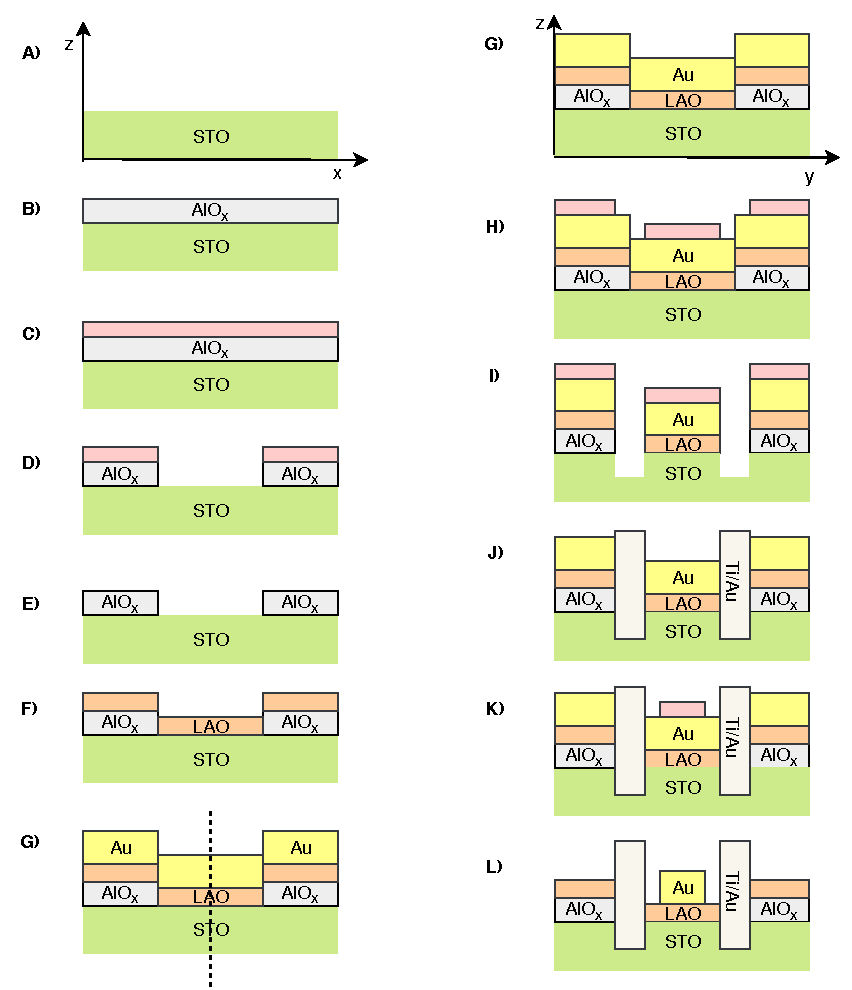
\includegraphics[scale = 1]{Figures/Fabrication.pdf}
    \caption{Fabrication steps for LAO/STO FET. Not drawn to scale.}
    \label{fig:fabrication_perfet}
\end{figure}

\pagebreak

\section{Percolation Simulation}
% model generated by uniformly distributed random number generator
% Under what assumptions you make so that this model is valid.
% mention how to find the shortest path using the path algorithm
% mention how each step is modelled extensions such as resistance between each nodes
% What measurement you did, in what setting, what number of cycles and the likes

A model to describe the percolative behaviour is made in the programming language Python. The code for this is discussed further in appendix A. In this model it is assumed that the plume from the PLD is uniformly distributed over the sample. In effect, the LAO patches can be assumed to be uniformly distributed throughout the sample. The metallic island is also assumed to be $\sim$\SI{100}{\nano\metre} in this simulation. Hence 1 site is equivalent to 100\si{nm}.

The simulation needs to be able to generate samples for different occupation density. This is defined as the occupation probability of the sample $p$ as stated in section \ref{section:Classical Percolation Theory}. To generate a sample under a $p$, an array is first initialized. The size of this array determines the size of the sample which can be set as a variable. Each element of the array is then filled by a pseudo-random number generator which samples a random real number from a uniform distribution over [0,1). Each element in the array is then compared to the occupation probability $p$. If the number of the element is smaller than $p$, the element would be set to 1 which signifies that it is an occupied site. Vice versa, the element will be set to 0 when it is bigger than $p$. Given the context of this report, an occupied site signifies that the LAO is 4 uc thick while an unoccupied site indicates that the LAO is 3 uc thick. 

To find the percolation threshold $p_c$, a search algorithm is implemented to check whether there is a percolating path between the edges of the sample in the Y-direction. An A* algorithm is implemented for this function. Further details about this algorithm is presented in appendix A. The algorithm itself is used to simply find the shortest percolating route from one end to another. Since the A* algorithm finds a path from a point to a point, the sample is padded with occupied sites in the top and bottom row as shown in figure \ref{fig:Simulation Sample figure}. This ensures that the algorithm can freely take any paths along the x-direction of the sample. The limitation of this simulation is that only lateral movements are allowed. Diagonal paths are not accounted for. Hence the algorithm only searches a path which leads from one occupied site to another nearest neighbour in the x or y direction.

$p_c$ is found numerically by sweeping $p$ of the sample from 0 to 1. The A* algorithm is used as a flag to indicate the existence of a percolating path. For each $p$, the experiment is done 20 times to reduce statistical errors. The algorithm will count how many times a percolating path exist given a certain $p$ over 20 tries. This number is then divided by 20 to give the probability of a percolating path $P_s$. Different sample size is also used in this experiment to see any effects caused by the finite size of the sample.

Simulation is also carried out to try to qualitatively replicate the behaviour of the phase transition of the sample. To observe the conductivity of such sample, it is assume here that each site gives a fix value of resistance, in this case 1 $\Omega$. Hence for each number of step, a higher resistance would be expected. The algorithm is also modified to find the 10 shortest independent paths that exist in the sample. This is done by marking the previous discovered path into an insulating path. This ensures that the algorithm will find the next shortest independent path. The same experiment is repeated by sweeping the occupation probability to find the relationship of the total resistance of the path and $p$. From the total resistance, conductivity can be calculated. From the same simulation, the number of paths vs the occupation probability can also be derived.

The RRTN can also be employed in the simulation by using the rules set in section \ref{section:RRTN}. By allowing a conductive path to exist between two metallic islands separated by an insulating gap, the RRTN can be considered. A variation in the voltage across the sample can also be done to investigate the phase transition behaviour in which tunneling current starts to occur.

\section{Device Characterization}

\begin{figure}[!t]
    \begin{minipage}{.5\linewidth}
    \centering
    \subfloat[]{\label{fig:Measurement_setup}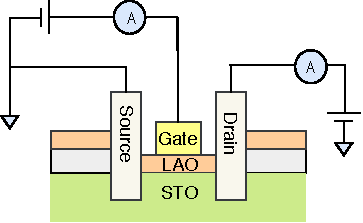
\includegraphics[scale = 1]{Figures/Measurement_Setup.pdf}}
    \end{minipage}
    \begin{minipage}{.5\linewidth}
    \centering
    \subfloat[]{\label{fig:equivalent_circuit}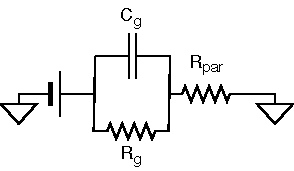
\includegraphics[scale = 1.1]{Figures/Equivalent_Circuit.pdf}}
    
    \end{minipage}\par\medskip
    \caption{(a) Measurement setup for I-V characterization of the device. (b) Equivalent circuit between for the C-V measurement.}
    \label{fig:Measurement Layout}
\end{figure}


\subsection{Transistor I-V Measurement}
Measurement of the FET is executed by using the probe station. In principle, the probe station uses metallic needles to make contacts with the FET's electrodes. Four probes are generally found in a setup which allows 4 contacts measurement. In this measurement only 3 probes are needed to make contacts at the drain, source, and gate electrodes. The sample is placed in a chamber that can be pressurized and cooled down.

The setup is shown in figure \ref{fig:Measurement_setup}. Labview is used to program both Keithley 2400 power supplies which are connected to the drain and the gate as shown in figure \ref{fig:Measurement_setup}. By using LabView, V\textsubscript{gs} and V\textsubscript{ds} can be varied accordingly. Current through the gate and drain is monitored via the Keithley power supplies.

The probe station allows measurement at both room temperature and at a low temperature of 10 K. For the V\textsubscript{gs} sweep, the gate voltage is swept back and forth from 0V to -2V and back to 1V ending back at 0V. Gate current and drain current are monitored accordingly. V\textsubscript{ds} is also incremented for every completed V\textsubscript{gs} sweep in steps of 100mV from -0.5V to 0.5V. As for the V\textsubscript{ds} sweep, the drain source voltage is swept in a similar fashion. V\textsubscript{ds} is swept from 0V to -0.5V and goes up to 5V and back to 0V in order to ensure that the saturation regime is observed. Likewise, for every completed V\textsubscript{ds} sweep, the V\textsubscript{gs} is incremented from -2.5V to 1V in steps of 100mV in order to investigate whether the device can be depleted.

A second test will be executed in low temperature and in the dark to reduce the generation of photocarriers \cite{hook_hall_2013}. The probe station chamber will be cooled down to 10K by helium flow. The pressure of the chamber is also kept at $\sim 10^{-6}$ bar. The same LabView program is run to characterize I-V curve of the device at low temperature.

In the case of low temperature measurement, the V\textsubscript{ds} is varied from -0.5V to 0.5V for the V\textsubscript{ds} sweep characterization. This ensures that the device does not overheat and distort the measurement at low temperatures due to the expected larger drain current because of mobility enhancement at lower temperatures \cite{caviglia}. Accordingly, for every completed sweep, V\textsubscript{gs} is incremented from -1.5V to 1.5V. In contrast, for the V\textsubscript{gs} sweep measurement, the gate voltage is varied from -1.5V to 1V and with V\textsubscript{ds} incremented from -0.5V to 5V. 

\subsection{C-V Measurement}\label{Sec:CV}
A Keithley 4200-SCS is used to measure the capacitance characteristics which can be later used to derive the mobility and the carrier density for the sample. This is done by measuring the complex, frequency-dependent impedance across the device by using a probe station. The device is similarly connected to figure \ref{fig:Measurement_setup} without the source connected to any contact. By applying a 50mV 10 KHz AC signal and a DC bias sweep at the gate, the impedance can be obtained and in turn the capacitance of the device can be calculated.

The equivalent circuit of the device is shown in figure \ref{fig:equivalent_circuit}. Here, the capacitance of the gate $C_g$ is in parallel with the gate resistance $R_g$. $R_{par}$ is accounted for the resistance of the 2DEG and other parasitic contribution. From the definition of impedance, it is known that it is divided into the resistance, R, and reactance, X, part expressed in equation \ref{eq:impedance}. This reactance consist of contributions made from the capacitance and inductance in the circuit. Given an impedance, the reactance can be calculated by using equation \ref{eq:reactance}. Where $\Theta$ is the phase difference introduced by the capacitor (for a purely capacitive contribution, phase shift is $-\pi/2$). From this value the reactance for a capacitance can be calculated by equation \ref{eq:Capacitor_reactance} where f is the frequency of the AC signal used during the measurement.

\begin{align}
    Z = R + jX \label{eq:impedance}\\ 
    X = |Z|\sin{\Theta}  \label{eq:reactance}\\
    X_c = \frac{1}{2\pi f C} \label{eq:Capacitor_reactance}
\end{align}

The choice of this frequency is critical. When a high frequency signal is used, the capacitive element would simply be a short circuit. Hence the gate capacitance can not be determined. In contrast, by using a relatively slow AC signal the capacitor would be an open circuit and only the series resistance $R_g$ and $R_{par}$ is measured. In this report, 10KHz was found suitable as the phase shift introduced was about  $-\pi/2$ which indicates that there is purely a resistive and capacitive element in the circuit.




\chapter{Result and Discussion}
The following section discusses about the results obtained from the annealed 4 uc LAO thick FET sample. Results for the sample without annealing is shown and discussed in appendix \ref{section:annealing appendix}. Room temperature and 10 K measurements are shown in two separate sections. For room temperature measurements, I-V characteristics, subthreshold swing, on-off ratio, capacitance characteristics, carrier density, and mobility measurements are shown. While the low temperature will only present the I-V characteristics, subthreshold swing, and on-off ratio. This 4 uc LAO/STO FET will also serves as a benchmark towards realizing the perFET. While the perFET has not been physically realized, a simulation study is performed to investigate how it will behave.

\section{Room Temperature Device Characteristic}
% Mention the E field in the gate, perhaps higher than conventional gate, 5Mv/cm?
% Gate current is several percentage of the drain current
% Show how to estimate Vds for higher temperature. based on the formula
% Adding dielectric on top of the gate, but that would be hard since you have to find an appropriate material with the right lattice constant, and properties which does not disrupt the polar discontinuities of the interface.
%The implementation of high-κ gate dielectrics is one of several strategies developed to allow further miniaturization of microelectronic components

% further analysis can be read from Ref \cite{percolation, christensen_2002, Stauffer_classical_percolation_2009}.

% gate thickness comparable to current technology. We want to ideally to improve transistors,
%huge reproducible hysteresis due to ionic fluctuation. No charge trapping since it shows that it does not keep that shape.
% Hysteresis, due to deep traps in the interface layer.

% From the fit, Vt = 0.3358181215957715. Which should be negative given that this is depletion type. A better fit would be a non integer exponent and a constant at constant. Fit reasonably well for lower voltages Vdsat but not higher.
% doping can be a problem, the concentration of doping becomes ineffective at smaller size scale mosfet. 


\subsection{V\textsubscript{ds} Sweep}
A V\textsubscript{ds} sweep measurement for an annealed 4 uc LAO/STO FET is shown in figure \ref{fig:Id Vs Vds dev16}. For this particular device, the FET has a gate area of 100\si{\micro m^{2}}.

Figure \ref{fig:Id Vs Vds dev16} shows that transistor operation is possible with LAO thickness of 4 uc. Both the ohmic regime and the saturation regime can be observed for different V\textsubscript{gs}. When V\textsubscript{gs} is - 1V, the device is seen to be fully depleted. Reproducible hysteresis is also seen when V\textsubscript{ds} is swept back and forth between -0.5V to 5V. 

V\textsubscript{d,sat} is marked in figure \ref{fig:Id Vs Vds dev16} by the blue dot. This is defined as V\textsubscript{gs}-V\textsubscript{t} in MOSFET term. At this point, pinch-off takes place in the drain contacts implying the transition from the ohmic regime to the saturation regime. The data points are then fitted by equation \ref{eq:saturation_eq}.

\begin{align}
    I_{d,sat} = \alpha(V_{gs} - V_t)^2 \label{eq:saturation_eq}
\end{align}

Where $\alpha$ is a proportionality constant and V\textsubscript{t} is the threshold voltage which is obtained as -1V from the I\textsubscript{d}-V\textsubscript{gs} measurement. The formula is derived based on the saturation regime of a MOSFET \cite{Semiconductor_explained_more}. It is observed that the V\textsubscript{d,sat} does not strictly scale quadratically. It is clear from the graph that at higher V\textsubscript{gs}, V\textsubscript{d,sat} is not located at between the ohmic and saturation regime. 


The explanation for the reproducible hysteresis observed in this measurement is possibly attributed from the depolarization of LAO due to large electric field. While concrete explanation is not available, further investigation towards this hysteresis can be done by taking different sweep rates. Observing whether higher sweep rate makes the hysteresis bigger can conclude that it is indeed due to the depolarization of LAO.

The observed non-quadratic behaviour of the I\textsubscript{d,sat} is due to the fact that the pinch-off mechanism happens differently in the 4 uc FET because the gate only covers the 2DEG partially unlike a MOSFET. In a typical MOSFET, the pinch-off point moves proportionally to V\textsubscript{d,sat} (i.e V\textsubscript{gs} - V\textsubscript{t}) due to the gate spanning along the channel. In this LAO/STO FET, the pinch-off point may not move proportionally to the V\textsubscript{d,sat} unless it is under the gate directly.


% Hence at more negative voltage, the depletion layer still grows towards the electrodes.

% Figure \ref{fig:Ig Vs Vds dev16} shows the leakage current of the device at different V\textsubscript{gs}. Leakage current as low as 10pA is observed during operation. At highly negative V\textsubscript{gs}, more leakage current is observed as the result of direct tunneling\cite{Peter_PHD_Thesis}. The main contribution of tunneling behaviour may be caused by the difference of large potential difference the gate and the drain contact. At V\textsubscript{gs}=-1V and V\textsubscript{ds}=5V, the potential difference between the drain and the gate is 6V. In contrast, when V\textsubscript{gs}=1V and V\textsubscript{ds}=5V, the voltage difference is 4V. Higher voltage difference leads to higher tunneling current. This explains the fact why the leakage current increases for a given V\textsubscript{gs}. 
 

\begin{figure}[!h]
    \centering
    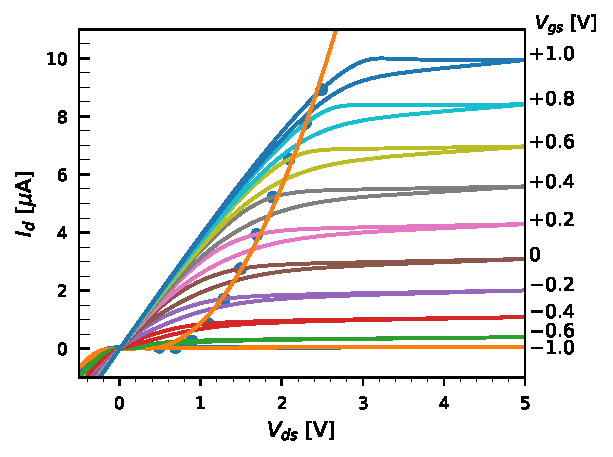
\includegraphics[scale=1]{Figures/Batch2/Dev16_batch2_Vds_sweep-Ids_With_Vdsat.pdf}
    \caption{I\textsubscript{d}-V\textsubscript{ds} plot of the 4 uc LAO/STO FET. The blue markers shown is where V\textsubscript{d,sat} occurs.}
    \label{fig:Id Vs Vds dev16}
\end{figure}


\newpage
\subsection{V\textsubscript{gs} Sweep}
Figure \ref{fig:Id Vs Vgs dev16} and \ref{fig:Ig Vs Vgs dev16} shows the result of the V\textsubscript{gs} sweep measurement on the same device. The measurement is also done under the same condition as the V\textsubscript{ds} measurement. 

The I\textsubscript{d}-V\textsubscript{gs} plot shows the transfer characteristic of the FET for positive V\textsubscript{ds}. It illustrates how the 2DEG forms when V\textsubscript{gs} is varied. The figure shows that I\textsubscript{d} increases with V\textsubscript{ds} as expected. The channel is found to be completely depleted when V\textsubscript{gs} = -1V indicating that the threshold voltage is -1V when Vgs is driven down to the negative value. The true exact value of the threshold voltage can not be determined directly as the device exhibits a memrisitive effect as shown. The threshold voltage of the device depends on the direction in which the V\textsubscript{gs} comes from. The subthreshold value and the on-off ratio can be calculated from this graph which is elaborated further in section \ref{sec:Sth-On/off RoomT}. 

Figure \ref{fig:Ig Vs Vgs dev16} shows how the gate leakage current varies with V\textsubscript{gs}. The sweep direction is also shown in the figure as black arrows. In the positive V\textsubscript{gs} direction, a diode like behaviour is observed. This is due to the quantum tunneling behaviour. At a sufficiently high V\textsubscript{gs}, the energy barrier of the LAO is thin enough that electrons can tunnel through. When the V\textsubscript{gs} is swept towards the negative side, the same thing happens. Tunneling current becomes more dominant as the energy barrier becomes thinner due to the 1.5\si{\nano\metre} dielectric thickness.

A unique behaviour is observed when the gate voltage is driven to the negative side. It is seen that the gate current reaches a maximum current (V\textsubscript{gs}=-1V) and starts to decrease when V\textsubscript{gs} goes even more negative. This phenomenon is also observed in the study done by Eerkes \cite{Peter_PHD_Thesis}. This phenomena is largely unexplored. But it is believed that this is due to the 2DEG being depleted through the gate. As the voltage gets negative, the 2DEG under the gate gets depleted hence gate current decreases. When more negative voltage is applied, the depleted 2DEG is not limited to under the gate. This depleted region extends further towards the electrodes. When the gate voltage is driven up to the positive side again, the 2DEG regenerates slowly hence the hysteresis \cite{Peter_PHD_Thesis, kim_kim_lim_jeong_kwon_baek_kim_2015}.

Memristive behaviour is also seen in figure \ref{fig:Id Vs Vgs dev16} similar to those found in ferroelectric FET devices \cite{wang_liu_2017}. A positive V\textsubscript{t} shift of 0.2V is observed during this measurement. This is phenomena may be attributed by the generation of deep traps at the LAO/STO interface at high negative voltage \cite{kim_kim_lim_jeong_kwon_baek_kim_2015} and due to the slowly regenerating 2DEG. When the device is fully depleted, the electrons may get trapped in the defects made from Ti\textsuperscript{+3} and Sr\textsuperscript{+2}\cite{yu_zunger_2014}. This effectively requires a higher amount of voltage to release them from the trap.

%not sure about the dip
%https://engineering.purdue.edu/~ee606/downloads/ECE606_f12_Lecture24.pdf
\begin{figure}[!t]
    \begin{minipage}{.5\linewidth}
    \centering
    \subfloat[]{\label{fig:Id Vs Vgs dev16}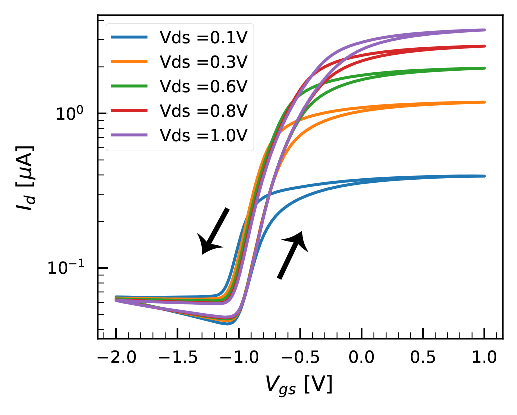
\includegraphics[scale =0.9]{Figures/Batch2/Dev16_batch2_Vgs_sweep-Ids(With_arrows).pdf}}
    \end{minipage}
    \begin{minipage}{.5\linewidth}
    \centering
    \subfloat[]{\label{fig:Ig Vs Vgs dev16}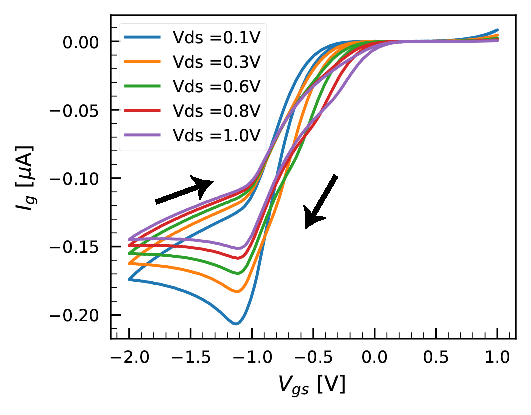
\includegraphics[scale = 0.9]{Figures/Batch2/Dev16_batch2_Vgs_sweep-Igs_(With_Arrows).pdf}}
    
    \end{minipage}\par\medskip
    \caption{(a) I\textsubscript{d}-V\textsubscript{gs} characteristics (b)I\textsubscript{g}-V\textsubscript{gs} characteristics. Black arrows shows the direction of the voltage sweep.}
    \label{fig:Vgs Sweep}
\end{figure}


\subsection{Subthreshold Swing and On-Off Ratio} \label{sec:Sth-On/off RoomT}
The subthreshold swing and the on-off ratio is derived from the I\textsubscript{d}-V\textsubscript{gs} characteristic. The subthreshold swing is obtained graphically by fitting a semi-log line (i.e $y = 10^{(mx+c)}$) through the data points around the maximum derivative of the graph between V\textsubscript{gs} of -1.1V to -0.8V. The value of the subthreshold swing can then be derived from the values of the semi-log fit and equation \ref{eq:Subthreshold swing numerical}. The on-off ratio is obtained by getting the value of I\textsubscript{d} at V\textsubscript{gs}=1 and I\textsubscript{d} at V\textsubscript{gs}=2. The result is shown in figure \ref{fig:Subth-OnOff-RoomTemp}. 

\begin{align}\label{eq:Subthreshold swing numerical}
    S = \frac{\Delta V_{gs}}{\Delta \log_{10}I_d}
\end{align}
From the figure, it can be seen that the on/off ratio linearly increases with V\textsubscript{ds}. The values indicates that the drain off current is still relatively large in comparison to the drain on current which is due to the leakage current for negative V\textsubscript{gs}. For a typical MOSFET, the on/off ratio is approximately $\sim 10^3-10^4$\cite{hu_2010} which is about two orders of magnitude higher than the device tested. Hence it can be concluded here that optimization of such device is still needed. In fact, it is perhaps better to have a thicker LAO layer to prevent lower leakage.

The subthreshold swing is also relatively high at 325mV/dec as the consequence of low on/off ratio. This is not ideal for low power transistor operations as it would mean that a relatively high amount of gate voltage is needed to change the drain current. 

\begin{figure}[!h]
    \centering
    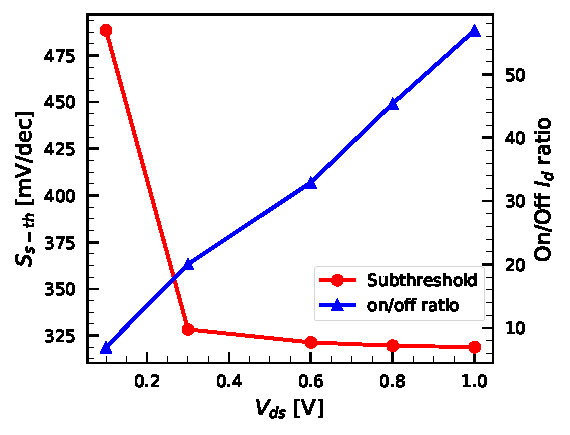
\includegraphics[scale=1]{Figures/Batch2/Dev16_batch2_Subth-on-off.pdf}
    \caption{Room temperature subthreshold swing and On/Off ratio}
    \label{fig:Subth-OnOff-RoomTemp}
\end{figure}

\newpage


\subsection{C-V characteristic}
The result of the C-V measurement of the same device at room temperature is shown in figure \ref{fig:CV_dev16}. This follows from the impedance measurement done between the gate and drain contacts (figure \ref{fig:Impedance_dev16}) with V\textsubscript{ds}=0V. It is observed from figure \ref{fig:Impedance_dev16} that the phase is approximately -90 degrees. This indicates that the reactance part of the impedance is contributed purely by a capacitive element. From the obtained impedance, the reactance and hence the capacitance can be calculated from following the method mentioned in section \ref{Sec:CV}. 

From figure \ref{fig:CV_dev16}, the oxide capacitance is obtained by taking the flat part of the graph at V\textsubscript{gs}=0.5V. From there, the capacitance was found to be approximately 4.2\si{pF}. Equivalently, the capacitance per unit area is 4.2 \si{\micro F/cm^2}. This result agrees considerably well with the value obtained by Stadhouder at 2.54\si{\micro F/cm^2} \cite{stadhouder_2018}. From the capacitance obtained from the measurement, the relative permittivity of LAO can be calculated. Given the assumption of a flat plate capacitor:

\begin{align}
    C = \frac{\epsilon_r \epsilon_0 A}{d}
\end{align}

Where A is area, d is thickness of the LAO layer, $\epsilon_0$ is the permittivity of free space, C is capacitance, and $\epsilon_r$ is the relative permittivity. $\epsilon_r$ is found to be 6.7 which is significantly lower than the value of $\epsilon_r$ in bulk LAO ($\sim$25) \cite{ohtomo_hwang_2004}. This variation in $\epsilon_r$ might be caused by dead layer \cite{hosoda_hikita_hwang_bell_2013} or some quantum capacitance effect \cite{li_Large_capacitance_enhancement_2011}.

More research should be done for this since the LAO/STO quantum capacitance enhancement is observed by Ref \cite{li_Large_capacitance_enhancement_2011}. This could benefit the device by having a subthreshold swing of lower than the classical 60mV/dec limit given that the capacitance can be negative due to the negative electron compressibility.

% From figure \ref{fig:CV_dev16}, the C-V characteristic resembles to those found for a p-MOSFET. The reason for this is while the channel is electrons, the V\textsubscript{gs} actually controls the holes in the device. The channel of electrons is an intrinsic property of the LAO/STO interface. To deplete such channel, effectively a channel of holes needs to be made by decreasing vgs to more negative. Still needs to be revised.



\begin{figure}
    \begin{minipage}{.5\linewidth}
    \centering
    \subfloat[]{\label{fig:Impedance_dev16}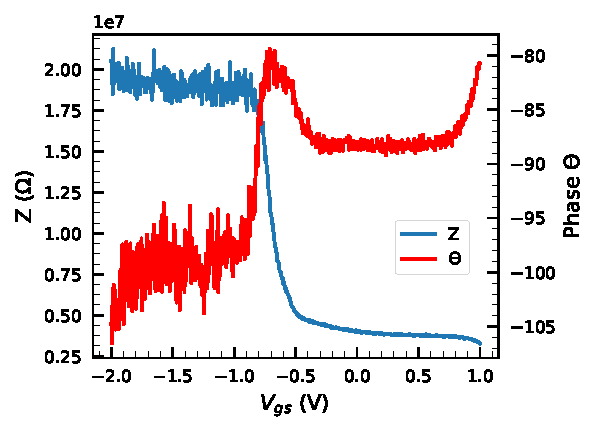
\includegraphics[scale =0.85]{Figures/CV/dev16-Impedance_10Khz.pdf}}
    \end{minipage}
    \begin{minipage}{.5\linewidth}
    \centering
    \subfloat[]{\label{fig:CV_dev16}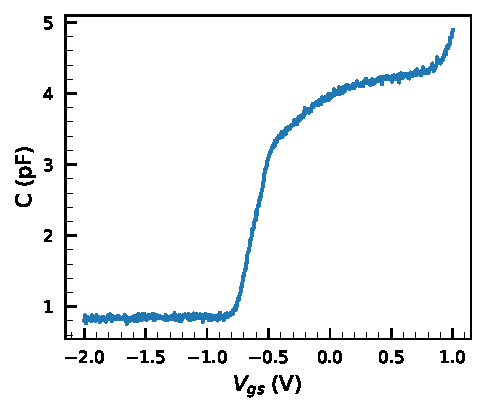
\includegraphics[scale = 0.85]{Figures/CV/dev16-CV-10KHz.pdf}}
    \end{minipage}\par\medskip
    \caption{(a) Impedance measurement of the device. Also shows the phase shift introduced by capacitive and inductive elements.(b) C-V characteristic of the device. At higher V\textsubscript{gs}, the 2DEG starts to form, hence an increase in capacitance.}
    \label{fig:CV_Impedance_figure}
\end{figure}

\subsection{Mobility and Carrier Density}
Given $\epsilon_r$, the mobility, $\mu$, and the carrier density, $n_s$, can be calculated following from the formula used by Ref \cite{eerkes_wiel_hilgenkamp_2013}.

\begin{align}
    n_s &= \frac{\epsilon_0 \epsilon_{r} V_{d,sat}}{e d}\\
    \mu &= 2\frac{I_{d,sat}d}{\epsilon_0 \epsilon_{r} V_{d,sat}^2} \frac{L}{W}
\end{align}


Where V\textsubscript{d,sat} and I\textsubscript{d,sat} are the voltage and the current at the saturation point, e as elementary charge, L as length of the channel,  W as the width of the channel, d is the thickness of the LAO layer, $\epsilon_0$ is the permittivity of free space,  and $\epsilon_r$ is the relative permittivity of the LAO.

V\textsubscript{d,sat} and I\textsubscript{d,sat} are extracted from the I\textsubscript{d}-V\textsubscript{ds} plot from figure \ref{fig:Id Vs Vds dev16}. By using the formulas, the mobility and the carrier density is calculated and plotted as illustrated in figure \ref{fig:mobility_carrier}. The result shows a comparatively close value to measurements obtained from other research \cite{thiel_2006,forg_richter_mannhart_2012,Peter_PHD_Thesis,hosoda_hikita_hwang_bell_2013}.

Based on the graph, a linear dependence on the carrier density is observed. This physically makes sense since higher V\textsubscript{gs} would attract more electrons. As mentioned before the value of $n_s$ is very much comparable to other reports at $\sim$$10^{13}$ \cite{caviglia, thiel_2006}. 

The mobility is shown to saturate at higher V\textsubscript{gs}. The mobility is calculated to be 7 \si{cm^2/Vs} at V\textsubscript{gs} $>$ 0.25V. For comparison, the value reported by other researches \cite{thiel_2006, kalabukhov_gunnarsson_2008} are between 5-10 \si{cm^2/Vs}. The intuitive reason behind this saturation of mobility is because that below V\textsubscript{gs}=0.25V, the 2DEG channel has not fully form yet.

\begin{figure}
    \centering
    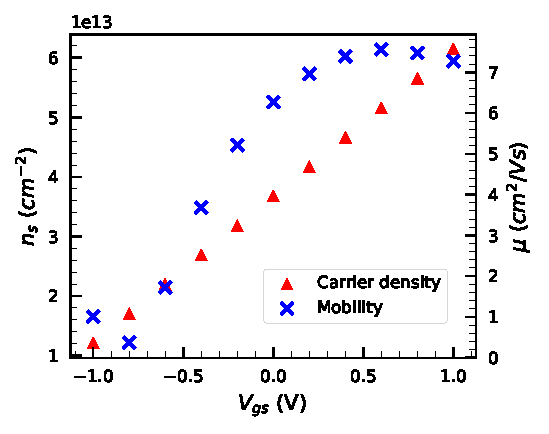
\includegraphics{Figures/CV/Mobility_and_Carrier_density.pdf}
    \caption{Mobility and carrier density plot for the 4 uc device}
    \label{fig:mobility_carrier}
\end{figure}



\section{Low Temperature Transistor I-V Curves}
\subsection{V\textsubscript{ds} Sweep}
The same device is now measured at 10K to observe the possibility of mobility enhancement and higher subthreshold swing. The I\textsubscript{d}-V\textsubscript{ds} characteristic is shown in figure \ref{fig:lowT_Vds_sweep-Ids}. The drain current shown is orders of magnitude higher than the ones observed in room temperature. Depletion characteristics are shown to be still visible at lower temperature for V\textsubscript{gs} below -0.5V. The device is depleted at -1V. Hysteresis also disappears in comparison to room temperature measurements. A non-symmetric behaviour at negative V\textsubscript{ds} is also shown in the graph similar to those found in the room temperature measurement. 

The higher drain current observed in figure \ref{fig:lowT_Vds_sweep-Ids} is caused by the enhancement of mobility at lower temperature which agrees with other studies \cite{caviglia,bogorin_irvin_cen_levy_2012}. The main reason for this enhancement can be originated from electron-phonon scattering as it is significantly less at low temperatures due to the limited movement of the nuclei \cite{hook_hall_2013}. In the same notion, the lack of hysteresis observed in the measurement is caused by the ionic compound freezing out at lower temperatures.

The non-symmetric behaviour seen at negative V\textsubscript{gs} can be explained by the intrinsic diode behaviour between the depleted region and the drain contact. The diode will only turn on once the potential difference between the gate and the drain is 1.1V. This also explains why there is a shift of this behaviour of 100mV for every 100mV variation of V\textsubscript{gs}.


\begin{figure}[!h]
    \centering
    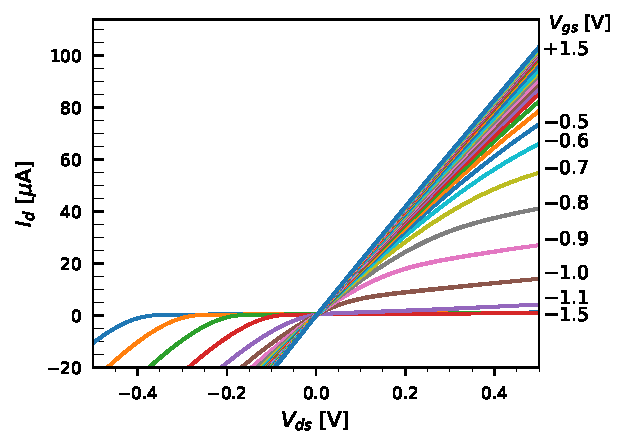
\includegraphics{Figures/LowT/Dev16_LowT_Vds_sweep-Ids}
    \caption{I\textsubscript{d}-V\textsubscript{ds} characteristics at 10K.}
    \label{fig:lowT_Vds_sweep-Ids}
\end{figure}

\subsection{V\textsubscript{gs} Sweep}
The I\textsubscript{d}-V\textsubscript{gs} characteristic of the FET is described in figure \ref{fig:lowT_Vgs_sweep-Ids}. Higher current is observed as expected. The threshold voltage seen from the characterization is the same as the room temperature measurement. What is different is that since the I\textsubscript{d,on} is higher than the room temperature measurement, the subthreshold swing of the FET is significantly lower. 

A dip is still observed from the I\textsubscript{d}-V\textsubscript{gs} characteristic regardless of the voltage sweep direction. The reason for this remains unclear which still needs further researched.

Figure \ref{fig:lowT_Vgs_sweep-Igs} shows the tunneling behaviour of the gate at low temperature. An exponential increase in leakage current is observed. This rectifying behaviour is expected as V\textsubscript{gs} becomes more negative. At negative V\textsubscript{gs}, a majority of holes resides on the interface of the LAO/STO replacing the 2DEG. At sufficient V\textsubscript{gs}, the barrier of the LAO dielectric is thin enough that the electrons from the gate can tunnel through the dielectric. This tunneling behaviour tends to be exponential which is what it is observed in figure \ref{fig:lowT_Vgs_sweep-Igs}.


\begin{figure}
    \begin{minipage}{.5\linewidth}
    \centering
    \subfloat[]{\label{fig:lowT_Vgs_sweep-Ids}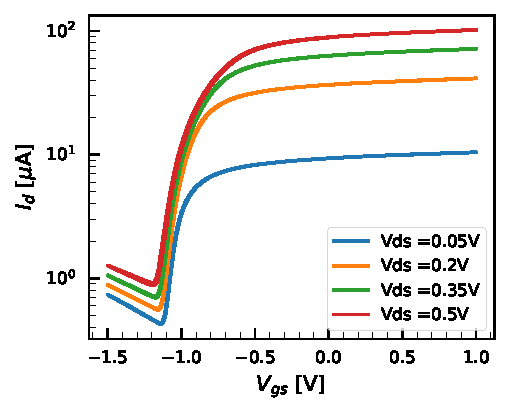
\includegraphics[scale =0.9]{Figures/LowT/Dev16_lowT_Vgs_sweep-Ids.pdf}}
    \end{minipage}
    \begin{minipage}{.5\linewidth}
    \centering
    \subfloat[]{\label{fig:lowT_Vgs_sweep-Igs}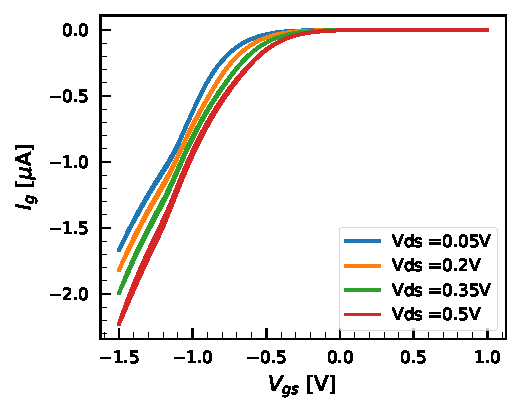
\includegraphics[scale = 0.9]{Figures/LowT/Dev16_lowT_Vgs_sweep-Igs.pdf}}
    
    \end{minipage}\par\medskip
    \caption{(a) Low temperature I\textsubscript{d}-V\textsubscript{gs} characteristics for positive V\textsubscript{ds}. (b) I\textsubscript{g}-V\textsubscript{gs} characteristics of the same device.}
    \label{fig:Vds Sweep}
\end{figure}

\subsection{Subthreshold Swing and On-Off ratio}
The subtreshold swing and the on-off ratio is calculated for transistor operation at 10K. This is defined identically to those found at room temperature. A better subthrehsold and on/off characteristic is obtained at lower temperature as shown in figure \ref{fig:lowT_subth}. A subthreshold swing of $\sim$100mV/dec is obtained from the low temperature measurement and it is comparable to a typical MOSFET. However, the on/off ratio is still not comparable to a typical MOSFET. Hence it may be recommendable to use a thicker LAO layer to reduce the direct tunneling leakage at the gate. 

A lower subthreshold swing is expected because of the T dependence on the subthreshold swing (See equation \ref{eq:subthreshold-swing}). Despite this, the subthreshold swing goal of less than 60mV/dec is not observed. Further research needs to be done to solve this problem. The reason why the subthreshold swing does not go below 60mV/dec is because the quantum capacitance increases with lower temperature and does not turn negative as it is initially thought \cite{li_Large_capacitance_enhancement_2011}.

The on/off ratio and the subthreshold swing can be improved further by operating the device at a lower temperature up to 300 mK. At this temperature, the 2DEG between in the interface becomes superconducting. It has been shown in several studies that this superconducting 2DEG can be modulated by an electrostatic field \cite{caviglia}. This modulation via the gate could in principle drive the phase transition between insulating and conducting state. This allows the possibility of increasing the on/off ratio of such device and subsequently enhance the subthreshold swing by having a higher I\textsubscript{ds,on}.


\begin{figure}[!h]
    \centering
    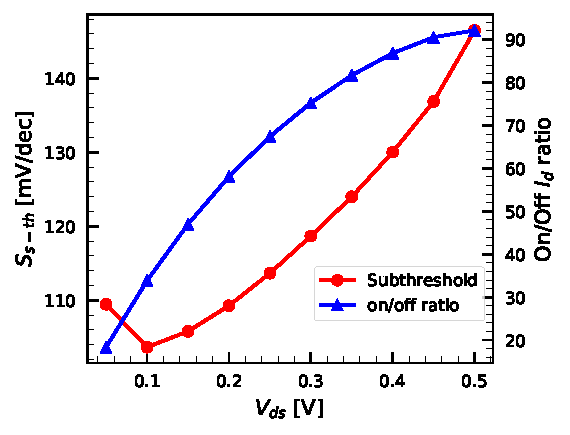
\includegraphics{Figures/LowT/Dev16_lowT_Subth-on-off.pdf}
    \caption{Subthreshold swing and on/off ratio versus V\textsubscript{ds} at lower 10K.}
    \label{fig:lowT_subth}
\end{figure}

\newpage

\section{Simulation}
A simulation study is conducted to study the behaviour a partially covered STO substrate by 4 uc of LAO dielectric. This would help to gain further insights to qualitatively describe the behaviour of a percolative FET. A study on the required LAO coverage density is also executed which can be helpful for the fabrication. 

The simulation is executed following from the methods in explained in Chapter 2. The result of the percolative simulation is summarized in figure \ref{fig:percolation_sim}. A more detail results on a 100x100 sample is shown in appendix section \ref{section:simulation_result}.

The relationship between the occupation probability of the sample $p$ and the probability of a spanning cluster $P_s$ is shown in figure \ref{fig:percprob-ocprob}. This is done to find the percolation threshold $p_c$. As one can see, the finite size of the sample is an important variable to consider. For a smaller sample, the percolation threshold $p_c$ is not well defined. But as the sample gets bigger, $P_s$ starts to behave like a step function and hence $p_c$ is well defined. The percolation threshold was found to be approximately at 0.59 based on numerical data. From this, it can be concluded that the size of the device matters. 

For the simulation, the algorithm will find 100 independent paths across a 100x100 sample. The simulation is repeated 10 times of each $p$ over the range of 0.5 to 1. The results are averaged to reduce statistical errors. From the simulation, it is observed that the number of independent paths found on the sample grows exponentially in comparison to the occupation probability as shown in figure \ref{fig:OcProb-NumPaths}. Moreover, the resistance of the sample shows that for an increasing number of paths, the resistance drops at 1/N (Figure \ref{fig:Numpaths-Resistance}). Most interestingly, a phase transition behaviour is observed shown in figure \ref{fig:OcProb-Conduct} based on occupation probability alone. It is shown that the sample will start conducting as expected when the occupation probability is above 0.59. It is noticed that the conductivity rapidly increase until $p=0.7$ and stars to slow down and monotonically increase. Hence it is maybe beneficial to actually aim for a 3.7 LAO thickness. 

To model the electrical behaviour of the perFET, several additional theories needs to be considered. Random resistor tunneling network can be incorporated with the model. An initial framework has been done during this project and the result is shown in figure \ref{fig:RRTN_simulation_result}. In this model, the non-linear I-V behaviour of the tunneling is not yet incorporated. However, an effective decrease in $p_c$ can already be observed when RRTN is considered geometrically. This is done by assuming that tunneling can occur between two islands when isolated by one insulating gap. When RRTN is considered, the percolation threshold $p_c$ will effectively be lower. This lowering of $p_c$ is caused by the lowering of the energy barrier based when a voltage difference is applied between the top and bottom of the sample (i.e V\textsubscript{ds}). As one can see from figure \ref{fig:RRTN_Sample}, there exist a percolative path between the two ends despite the $p$ of the sample is set to 0.4. Without RRTN, the sample would have no percolating path as shown in figure \ref{fig:non_RRTN}.

Another alternative way to model the perFET is by modelling the gate capacitance behaviour of the device. One way to do so is to calculate the size of the percolating cluster by using Hoshen-Kopelman algorithm \cite{percolation_simulation}. By measuring the size of the cluster, an equivalent area for the gate capacitance can be calculated. A charge based simulation can be done similarly to those used for MOSFET simulation \cite{Semiconductor_explained_more}.

Further investigation is needed to fully realized the perFET. The effect of the drain-source and the gate voltage should also be considered due to the non-homogeneous electric field as the result of percolative interface. A percolative device has been demonstrated by Li \cite{li_graf_schladt_jiang_parkin_2012} by using electrolyte and STO substrate. The behaviour shows promise that it does indeed undergoes phase transition for a given V\textsubscript{ds}. Hence, it is compelling to see what happens when the electrolyte solution used in that research is substituted with partial patches of 4 uc of LAO.

\begin{figure}[!h]
\begin{minipage}{.5\linewidth}
\centering
\subfloat[]{\label{fig:percprob-ocprob}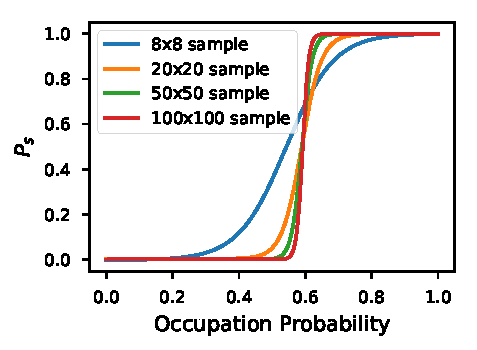
\includegraphics{Figures/percprob_vs_occprob.pdf}}
\end{minipage}%
\begin{minipage}{.5\linewidth}
\centering
\subfloat[]{\label{fig:OcProb-NumPaths}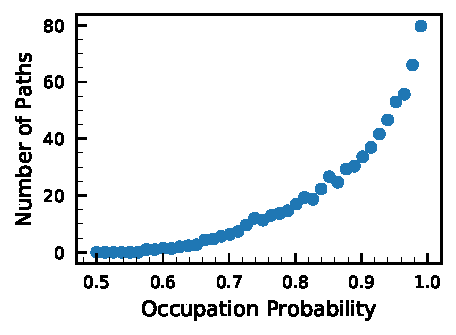
\includegraphics{Figures/OcProb-NumPaths.pdf}}
\end{minipage}\par\medskip
\begin{minipage}{.5\linewidth}
\centering
\subfloat[]{\label{fig:Numpaths-Resistance}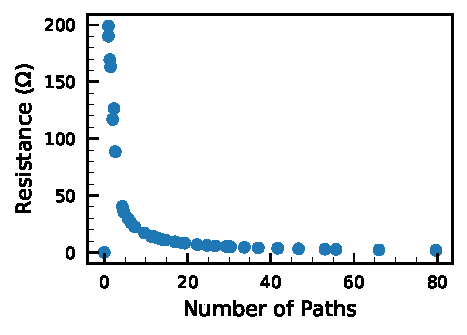
\includegraphics{Figures/NumPaths-Resistance.pdf}}
\end{minipage}%
\begin{minipage}{.5\linewidth}
\centering
\subfloat[]{\label{fig:OcProb-Conduct}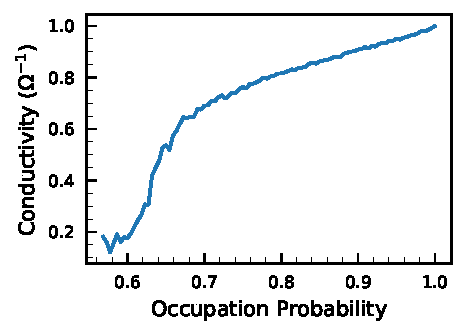
\includegraphics{Figures/OcProb-Conduct.pdf}}
\end{minipage}%

\caption{Result of the simulation for 100x100 grid.(a) Occupation probability and percolation probability characteristics. A step function is formed as the sample size goes to infinity (b) Number of paths found in the sample in relation with the occupation probability.(c) 1/N dependence of resistance relationship with the number of paths found.(d) Normalized conductivity of the sample with respect to occupation probability.}
\label{fig:percolation_sim}
\end{figure}

\newpage
\begin{figure}[t!]
\begin{minipage}{.5\linewidth}
\centering
\subfloat[]{\label{fig:non_RRTN}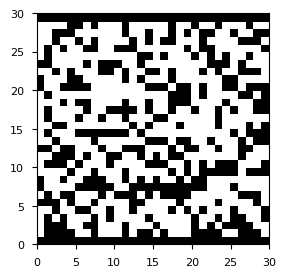
\includegraphics[width = 0.75\textwidth]{Figures/non_RRTN_appendix.png}}
\end{minipage}
\begin{minipage}{.5\linewidth}
\centering
\subfloat[]{\label{fig:RRTN_Sample}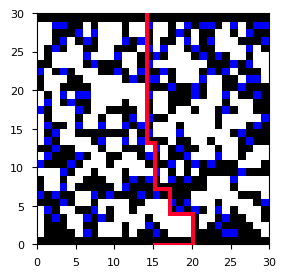
\includegraphics[width = 0.75\textwidth]{Figures/RRTN_percolative.png}}

\end{minipage}\par\medskip
\caption{30x30 Sample with $p$ = 0.4. (a) Non-RRTN sample. (b) RRTN sample. A percolative path is found for an RRTN sample, but not on the non-RRTN sample. Blue squares indicate paths that are available through tunneling.}\label{fig:RRTN_simulation_result}
\end{figure}






\chapter{Conclusion}
In conclusion, we demonstrate that LAO/STO FET is still operable by using LAO thickness of 4 unit cells. Device characterization has shown that the field effect transistor behave similarly to a MOSFET to a certain extent. Both the ohmic and saturation regime can be observed. It is shown from experiments that the 2DEG from the LAO/STO interface can be fully depleted in both room temperature and at 10K. The 4 uc FET however does not have the same V\textsubscript{d,sat} as predicted from the MOSFET equation. The measurement also indicates an enhancement of drain current in lower temperature is in agreement with other studies. The mobility and the carrier density is also quantified for this device and it is in accordance with other reports. Moreover, lower gate voltage is achieved by having a thinner LAO layer. Despite this, the leakage current becomes more prominent in the device. Thus, effecting the subtheshold swing and subsequently the on/off ratio.

Unique characteristic is observed throughout the measurement of the 4 uc device. Indications of a very reproducible memristive effect is seen from the measurement despite LAO being non-ferroelectric.An explanation for this still needs to be further investigated. But we propose that the memristive effect is mostly caused by charge trapping in the LAO/STO interface due to defects in combination with the slowly regenerating 2DEG.

The perFET however still needs a lot of theory and testing to be fully utilized. Simulation suggests that 3.6 uc LAO coverage is enough to make a percolating path. When RRTN phenomenon is considered in the model, metal-insulator transition is expected due to external electric field. More research is still required regarding the influence of V\textsubscript{ds} and V\textsubscript{gs} on the phase transition of the percolative channel. 

On the basis of the 4 uc device, it is expected that the perFET will have a higher leakage current and a lower threshold voltage. To eventually realize a percolation based FET, another material may be needed to be deposit on top of the 4 uc LAO layer. With a thicker dielectric layer, the tunneling current is hopefully reduced.

\newpage
\section*{Outlook}
Device characterization shows that the 4 uc LAO/STO FET needs more optimization. But it can be said from the research that thicker dielectric thickness may be preferable. While lower V\textsubscript{gs} is achieved, tunneling current becomes problematic. Hence more research needs to be done to minimize this effect.

An interesting research that can be conducted is also the combination of short channel length on LAO/STO based transistor \cite{woltmann_harada_boschker_srot_aken_klauk_mannhart_2015} and thin LAO layers. This will allow to fully characterize the LAO/STO FET scaling properties which is beneficial for minituarizing the LAO/STO based FET.

A study of quantum capacitive enhancement can also be investigated for this device. This study will help to optimize the subthreshold swing. In a view of Ref \cite{li_Large_capacitance_enhancement_2011}, quantum capacitance can turn negative which ultimately lowers the subthreshold swing below the classical 60mV/dec at room temperature.

To fully realize a perFET, more simulation work needs to be done. An alternative way of simulating the FET is by using capacitance based model as mentioned in the result. To actually fabricate a perFET, an additional layer of dielectric may be used on top of the LAO layer. But care must be taken, an appropriate material needs to be chosen carefully in order to not change the behaviour of the LAO/STO interface. 

\appendix
\chapter{Simulations}
The full simulation program along with the weekly journal for this project can be found in the Jupyter Notebook: \url{https://nbviewer.jupyter.org/github/prabowobagas/perFET/blob/master/Weekly\%20Journal.ipynb}.

\section{A* Algorithm}
A* (A star) algorithm is based on the Dijkstra's algorithm. While the Dijkstra algorithm finds all the paths leading to several different points, the A* algorithm finds a path between 2 points by means of heuristic comparison. The pseudo-code of this implementation is shown below. This is based on Ref \cite{A*search}.

The A* algorithm decides where to go based on equation \ref{eq:a*}. The algorithm decides which cell will be visited based on the lowest f(n). In principle, the A* initially scans the adjacent nodes from starting point. Each cell is evaluated whether it is closer to the point of destination or not. If it is, then the neighbouring node will become the current node. The node will then check it's adjacent cell again and remembers where it has been. The checked nodes is stored in the closed list. While the openlist stores the path where the algorithm has been.

\begin{align}\label{eq:a*}
    f(n) = g(n) + h(n)
\end{align}
Where:
f(n) = \text{total estimate cost of path through node n}\\
g(n) = \text{Cost so far to reach node n}\\
h(n) = \text{Estimated cost from n to goal. Usually $h(n)=\sqrt{(X_{goal}-X_{start})^2 + (Y_{goal}-Y_{start})^2}$}


\begin{lstlisting}[language=Python]
   make an openlist containing only the starting node
   make an empty closed list

   while (the destination node has not been reached):
       consider the node with the lowest f score in the open list
       if (this node is our destination node) :
           we are finished 
       if not:
           put the current node in the closed list and look at all of its neighbors
           for (each neighbor of the current node):
               if (neighbor has lower g value than current and is in the closed list) :
                   replace the neighbor with the new, lower, g value 
                   current node is now the neighbor's parent            
               else if (current g value is lower and this neighbor is in the open list ) :
                   replace the neighbor with the new, lower, g value 
                   change the neighbor's parent to our current node

               else if this neighbor is not in both lists:
                   add it to the open list and set its g
\end{lstlisting}

\section{Simulation Result}\label{section:simulation_result}
Several different occupation probability is shown in figure \ref{fig:sample_visualized}. The figures visualize the phase change of the sample as occupation probability increase. A change in phase is observed in figure \ref{fig:sample_visualized}b when a conductive path is found at $p=0.6$. As the occupation probability increase, more paths are found. Here, only the 10 shortest independent paths is calculated. The reason is that it is impossible to simulate all the possible conductive path in the sample as there are extremely many combinations. As one can see, as the occupation probability increases, the overall path length becomes shorter hence physically, the mobility of the electron becomes higher and the resistance effectively becomes lower. As occupation probability becomes higher, more paths are found too when the 10 independent path limit is set to a higher number.

\begin{figure}[!ht]
\centering
    \subfloat[p=0.5]{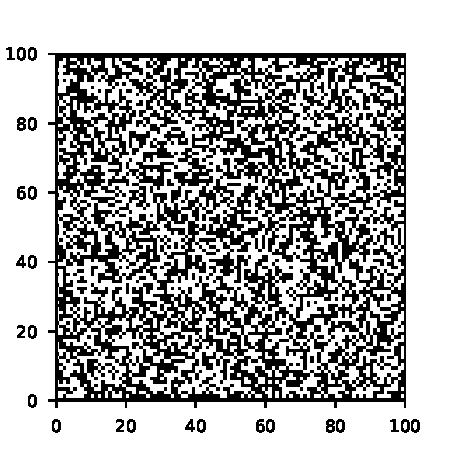
\includegraphics[width=0.45\linewidth]{Figures/Sample/pc-05.pdf}}
\hfil
    \subfloat[p=0.6]{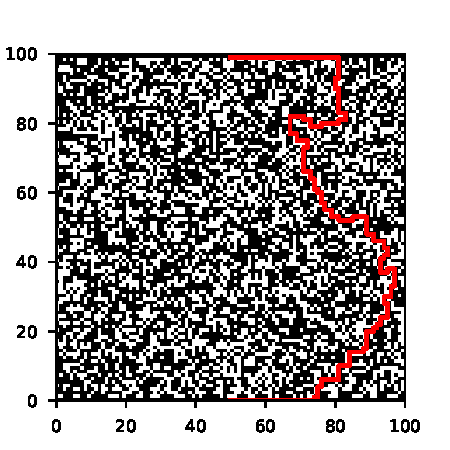
\includegraphics[width=0.45\linewidth]{Figures/Sample/pc-06.pdf}}

    \subfloat[p=0.7]{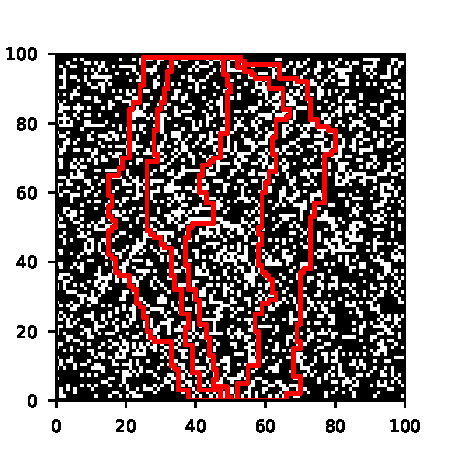
\includegraphics[width=0.45\linewidth]{Figures/Sample/pc-07.pdf}}
\hfil
    \subfloat[p=0.8]{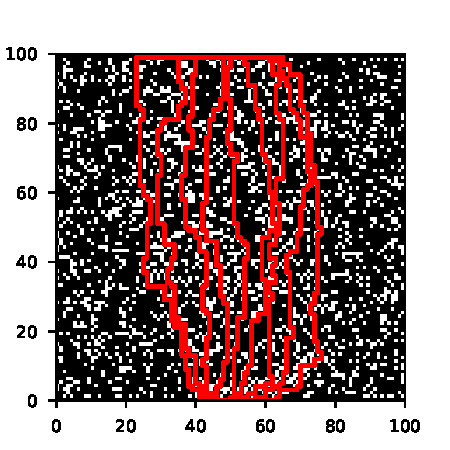
\includegraphics[width=0.45\linewidth]{Figures/Sample/pc-08.pdf}}

    \subfloat[p=0.9]{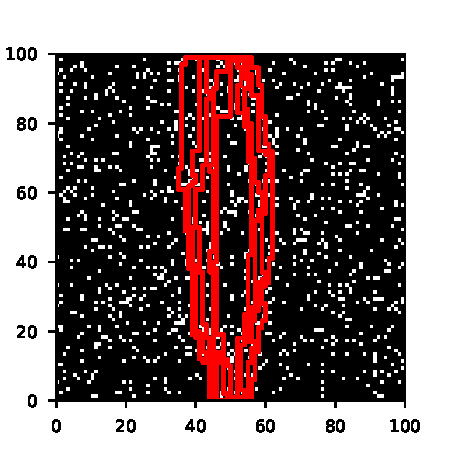
\includegraphics[width=0.45\linewidth]{Figures/Sample/pc-09.pdf}}
\hfil
    \subfloat[p=0.99]{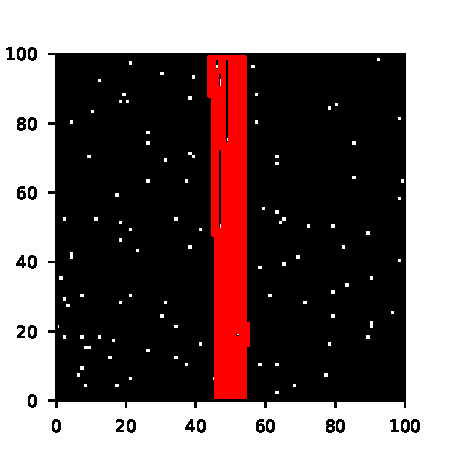
\includegraphics[width=0.45\linewidth]{Figures/Sample/pc-099.pdf}}
\caption{100 x 100 grid percolation simulation with different occupation probability p. Simulation shows the 10 shortest path that exist in the sample.}
\label{fig:sample_visualized}
\end{figure}

\chapter{Effects of Annealing on LAO/STO FET}\label{section:annealing appendix}
During the course of this project, a sample of 4 uc LAO/STO FET is treated without annealing. This can be served as a benchmark to the other annealed sample which is used in this report. This following section shows the I-V characterization of such sample. The measurement setup is identical to the ones reported. Measurement is done in room temperature and not enclosed in the dark. The measured device in this section has a gate area of 100\si{\micro m^{2}} which is identical to the ones reported.

\section{Results}
I\textsubscript{d}-V\textsubscript{ds} of the sample is shown in figure \ref{fig:Appendix-Id Vs Vds dev16}. The result shows that it has higher drain current in comparison the the sample reported. Just like the annealed sample, the FET can be depleted at room temperature. Clear ohmic and saturation regime is observed. The sample also shows that the V\textsubscript{d,sat} does not strictly obey the quadratic behaviour found in a MOSFET. 

\begin{figure}[!h]
    \centering
    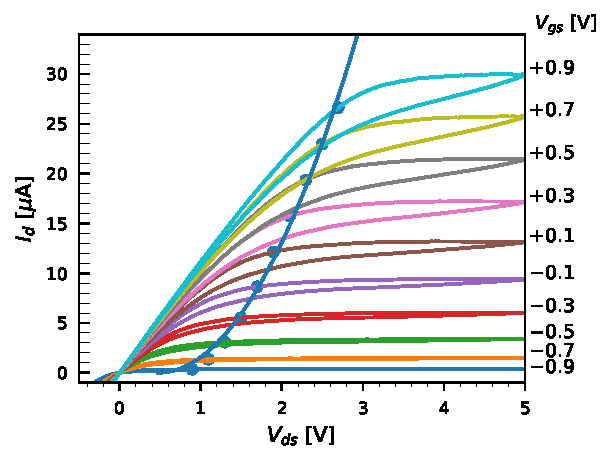
\includegraphics[scale=1]{Figures/Batch1/Dev16_Vds_sweep-Ids.pdf}
    \caption{I\textsubscript{d}-V\textsubscript{ds} plot of the non-annealed 4 uc LAO/STO FET. The blue markers shown is where V\textsubscript{d,sat} occurs.}
    \label{fig:Appendix-Id Vs Vds dev16}
\end{figure}

Figure \ref{fig:Appendix-Id Vs Vgs dev16} and figure \ref{fig:Appendix-Ig Vs Vgs dev16}
\begin{figure}
    \begin{minipage}{.5\linewidth}
    \centering
    \subfloat[]{\label{fig:Appendix-Id Vs Vgs dev16}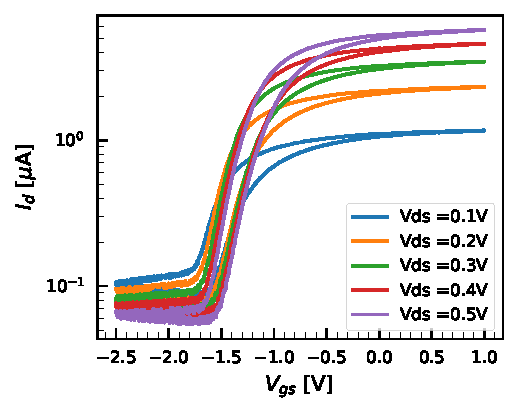
\includegraphics[scale =0.9]{Figures/Batch1/Dev16_Vgs_sweep-Ids.pdf}}
    \end{minipage}
    \begin{minipage}{.5\linewidth}
    \centering
    \subfloat[]{\label{fig:Appendix-Ig Vs Vgs dev16}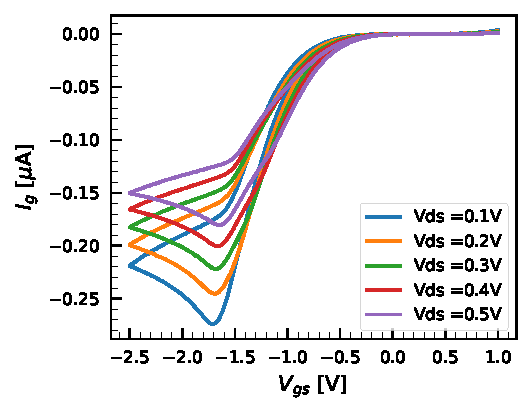
\includegraphics[scale = 0.9]{Figures/Batch1/Dev16_Vgs_sweep-Igs}}
    
    \end{minipage}\par\medskip
    \caption{(a) I\textsubscript{d}-V\textsubscript{gs} characteristics (b)I\textsubscript{g}-V\textsubscript{gs} characteristics. Black arrows shows the direction of the voltage sweep.}
    \label{fig:Appendix-Vgs Sweep}
\end{figure}


\begin{figure}
    \centering
    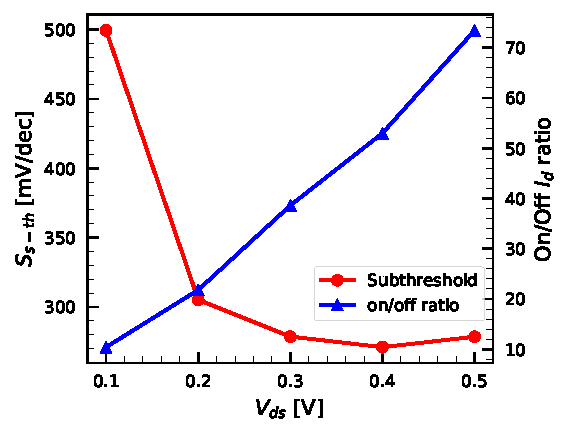
\includegraphics[scale=1]{Figures/Batch1/Dev16_Subth-on-off.pdf}
    \caption{Subthreshold swing and on/off ratio performance of the same device}
    \label{fig:Appendix-SS-Onoff}
\end{figure}


\section{Discussion}


\nocite{*}
\printbibliography


\end{document}
